% LukeO rip-off
\tikzstyle{c_mirgecom}   = []
\tikzstyle{c_meshmode}   = []
\tikzstyle{c_grudge}     = []
\tikzstyle{c_loopy}      = []
\tikzstyle{c_pytato}     = []
\tikzstyle{c_pyopencl}   = []
\tikzstyle{c_modepy}     = []
\tikzstyle{c_pymbolic}   = []
\tikzstyle{c_pocl}       = []
\tikzstyle{c_arraycontext} = []
\newcommand{\softwaredeps}{
  \tikzstyle{every path} = [line width=0.3pt,black!70]
  \tikzstyle{every node} = [scale=1.5,IllinoisBlue, line width=1pt]
  \begin{tikzpicture}[>=latex',line join=bevel,scale=0.34,
                      transform shape]
      %%
\node (mirgecom) at (306.3bp,522.0bp) [draw,ellipse,c_mirgecom] {mirgecom};
  \node (meshmode) at (198.3bp,378.0bp) [draw,ellipse,c_meshmode] {meshmode};
  \node (grudge) at (275.3bp,450.0bp) [draw,ellipse,c_grudge] {grudge};
  \node (loopy) at (300.3bp,162.0bp) [draw,ellipse,c_loopy] {loopy};
  \node (pytato) at (398.3bp,234.0bp) [draw,ellipse,c_pytato] {pytato};
  \node (pyopencl) at (82.3bp,90.0bp) [draw,ellipse,c_pyopencl] {pyopencl};
  \node (modepy) at (194.3bp,306.0bp) [draw,ellipse,c_modepy] {modepy};
  \node (arraycontext) at (82.3bp,306.0bp) [draw,ellipse,c_arraycontext] {arraycontext};
  \node (pymbolic) at (339.3bp,90.0bp) [draw,ellipse,c_pymbolic] {pymbolic};
  \node (pocl) at (82.3bp,18.0bp) [draw,ellipse,c_pocl] {pocl};
  \draw [->] (mirgecom) ..controls (263.07bp,497.84bp) and (243.93bp,484.43bp)  .. (231.3bp,468.0bp) .. controls (217.23bp,449.7bp) and (208.68bp,424.78bp)  .. (meshmode);
  \draw [->] (mirgecom) ..controls (295.22bp,495.97bp) and (290.85bp,486.12bp)  .. (grudge);
  \draw [->] (mirgecom) ..controls (322.13bp,477.36bp) and (338.3bp,424.99bp)  .. (338.3bp,379.0bp) .. controls (338.3bp,379.0bp) and (338.3bp,379.0bp)  .. (338.3bp,305.0bp) .. controls (338.3bp,263.41bp) and (322.9bp,217.22bp)  .. (loopy);
  \draw [->] (mirgecom) ..controls (333.95bp,495.26bp) and (345.45bp,482.01bp)  .. (352.3bp,468.0bp) .. controls (386.02bp,399.05bp) and (395.02bp,307.18bp)  .. (pytato);
  \draw [->] (meshmode) ..controls (224.34bp,350.64bp) and (235.59bp,337.39bp)  .. (243.3bp,324.0bp) .. controls (256.77bp,300.58bp) and (279.94bp,228.93bp)  .. (loopy);
  \draw [->] (meshmode) ..controls (105.37bp,361.51bp) and (34.495bp,345.65bp)  .. (18.3bp,324.0bp) .. controls (-29.855bp,259.62bp) and (29.958bp,161.05bp)  .. (pyopencl);
  \draw [->] (meshmode) ..controls (196.87bp,351.98bp) and (196.34bp,342.71bp)  .. (modepy);
  \draw [->] (meshmode) ..controls (156.9bp,352.02bp) and (134.42bp,338.45bp)  .. (arraycontext);
  \draw [->] (grudge) ..controls (248.31bp,424.47bp) and (234.95bp,412.31bp)  .. (meshmode);
  \draw [->] (grudge) ..controls (280.96bp,384.29bp) and (292.77bp,249.18bp)  .. (loopy);
  \draw [->] (loopy) ..controls (237.05bp,140.69bp) and (169.33bp,118.95bp)  .. (pyopencl);
  \draw [->] (loopy) ..controls (314.0bp,136.4bp) and (319.79bp,126.02bp)  .. (pymbolic);
  \draw [->] (pyopencl) ..controls (82.3bp,63.983bp) and (82.3bp,54.712bp)  .. (pocl);
  \draw [->] (arraycontext) ..controls (146.51bp,263.17bp) and (228.67bp,209.66bp)  .. (loopy);
  \draw [->] (arraycontext) ..controls (82.3bp,250.83bp) and (82.3bp,163.18bp)  .. (pyopencl);
  \draw [->] (arraycontext) ..controls (130.09bp,291.77bp) and (137.92bp,289.77bp)  .. (145.3bp,288.0bp) .. controls (219.86bp,270.15bp) and (307.59bp,252.52bp)  .. (pytato);
  \draw [->] (pytato) ..controls (364.12bp,208.58bp) and (343.5bp,193.86bp)  .. (loopy);
  \draw [->] (pytato) ..controls (381.14bp,191.71bp) and (362.22bp,146.17bp)  .. (pymbolic);
%

  \end{tikzpicture}
}
%\newcommand{\softwaredeps}{
%  \tikzstyle{every path} = [thick,black]

\begin{tikzpicture}[>=latex',line join=bevel,scale=0.5,transform shape]
  \node[c_mirgecom] (mirgecom) at (128.0bp,394.0bp) [draw,ellipse] {mirgecom};
  \node[c_meshmode] (meshmode) at (66.0bp,250.0bp) [draw,ellipse] {meshmode};
  \node[c_grudge] (grudge) at (101.0bp,322.0bp) [draw,ellipse] {grudge};
  \node[c_loopy] (loopy) at (165.0bp,178.0bp) [draw,ellipse] {loopy};
  \node[c_pytato] (pytato) at (206.0bp,250.0bp) [draw,ellipse] {pytato};
  \node[c_pyopencl] (pyopencl) at (89.0bp,106.0bp) [draw,ellipse] {pyopencl};
  \node[c_modepy] (modepy) at (56.0bp,178.0bp) [draw,ellipse] {modepy};
  \node[c_pymbolic] (pymbolic) at (194.0bp,106.0bp) [draw,ellipse] {pymbolic};
  \node[c_pocl] (pocl) at (89.0bp,34.0bp) [draw,ellipse] {pocl};
  \draw [->] (mirgecom) ..controls (83.575bp,370.85bp) and (65.825bp,357.6bp)  .. (57.0bp,340.0bp) .. controls (47.309bp,320.67bp) and (50.82bp,296.05bp)  .. (meshmode);
  \draw [->] (mirgecom) ..controls (118.38bp,368.06bp) and (114.63bp,358.33bp)  .. (grudge);
  \draw [->] (mirgecom) ..controls (137.95bp,365.74bp) and (142.3bp,352.27bp)  .. (145.0bp,340.0bp) .. controls (155.24bp,293.54bp) and (160.68bp,238.3bp)  .. (loopy);
  \draw [->] (mirgecom) ..controls (145.03bp,365.67bp) and (153.18bp,352.19bp)  .. (160.0bp,340.0bp) .. controls (171.75bp,319.0bp) and (184.24bp,294.7bp)  .. (pytato);
  \draw [->] (meshmode) ..controls (102.68bp,223.07bp) and (122.14bp,209.3bp)  .. (loopy);
  \draw [->] (meshmode) ..controls (90.689bp,223.14bp) and (100.44bp,209.89bp)  .. (105.0bp,196.0bp) .. controls (111.74bp,175.46bp) and (106.6bp,151.26bp)  .. (pyopencl);
  \draw [->] (meshmode) ..controls (62.426bp,223.98bp) and (61.102bp,214.71bp)  .. (modepy);
  \draw [->] (grudge) ..controls (88.625bp,296.25bp) and (83.61bp,286.22bp)  .. (meshmode);
  \draw [->] (grudge) ..controls (113.31bp,293.86bp) and (119.52bp,280.15bp)  .. (125.0bp,268.0bp) .. controls (134.58bp,246.76bp) and (145.41bp,222.66bp)  .. (loopy);
  \draw [->] (loopy) ..controls (138.91bp,152.97bp) and (125.17bp,140.32bp)  .. (pyopencl);
  \draw [->] (loopy) ..controls (175.22bp,152.34bp) and (179.32bp,142.43bp)  .. (pymbolic);
  \draw [->] (pyopencl) ..controls (89.0bp,79.983bp) and (89.0bp,70.712bp)  .. (pocl);
  \draw [->] (pytato) ..controls (191.47bp,224.19bp) and (185.2bp,213.49bp)  .. (loopy);
  \draw [->] (pytato) ..controls (207.38bp,213.92bp) and (207.7bp,184.89bp)  .. (205.0bp,160.0bp) .. controls (204.07bp,151.46bp) and (202.41bp,142.26bp)  .. (pymbolic);
  %\draw[red!50] (0,0) rectangle (230pt, 387.0pt);
\end{tikzpicture}

%}
\begin{frame}\frametitle{Outline}
\begin{minipage}[T]{0.45\textwidth}
  \begin{itemize}
    \item MIRGE-Com Overview
    \item Performance \& Scalability
    \item Code Challenges
    %    \begin{itemize}
    %        \item Partitioning \& DAG Splat Issues
    %        \item Mesh Processing Complexities (dont forget about enhanced instrumentation)
    %        \item DAG Complexity with physics development/capabilities
    %        \item Upcoming Threats \& Concerns
    %    \end{itemize}
    %  \end{itemize}
    \item Conclusion \& Future Directions
    %\begin{itemize}
    %    \item Upcoming Review Priorities
    %    \item Vision \& Long-Term Goals
    %\end{itemize}
  \end{itemize}
\end{minipage}
\hfill
\begin{minipage}[T]{0.45\textwidth}
  \centering
  \tikzstyle{c_mirgecom}=[draw=myOrange, line width=0.5mm]
  \softwaredeps%
\end{minipage}
  \url{https://github.com/illinois-ceesd/mirgecom/}
\end{frame}

\begin{frame}
    \centering
    \Large
    MIRGE-Com in Y3
\end{frame}

\begin{frame}\frametitle{Architecture Overview}
  \begin{center}
  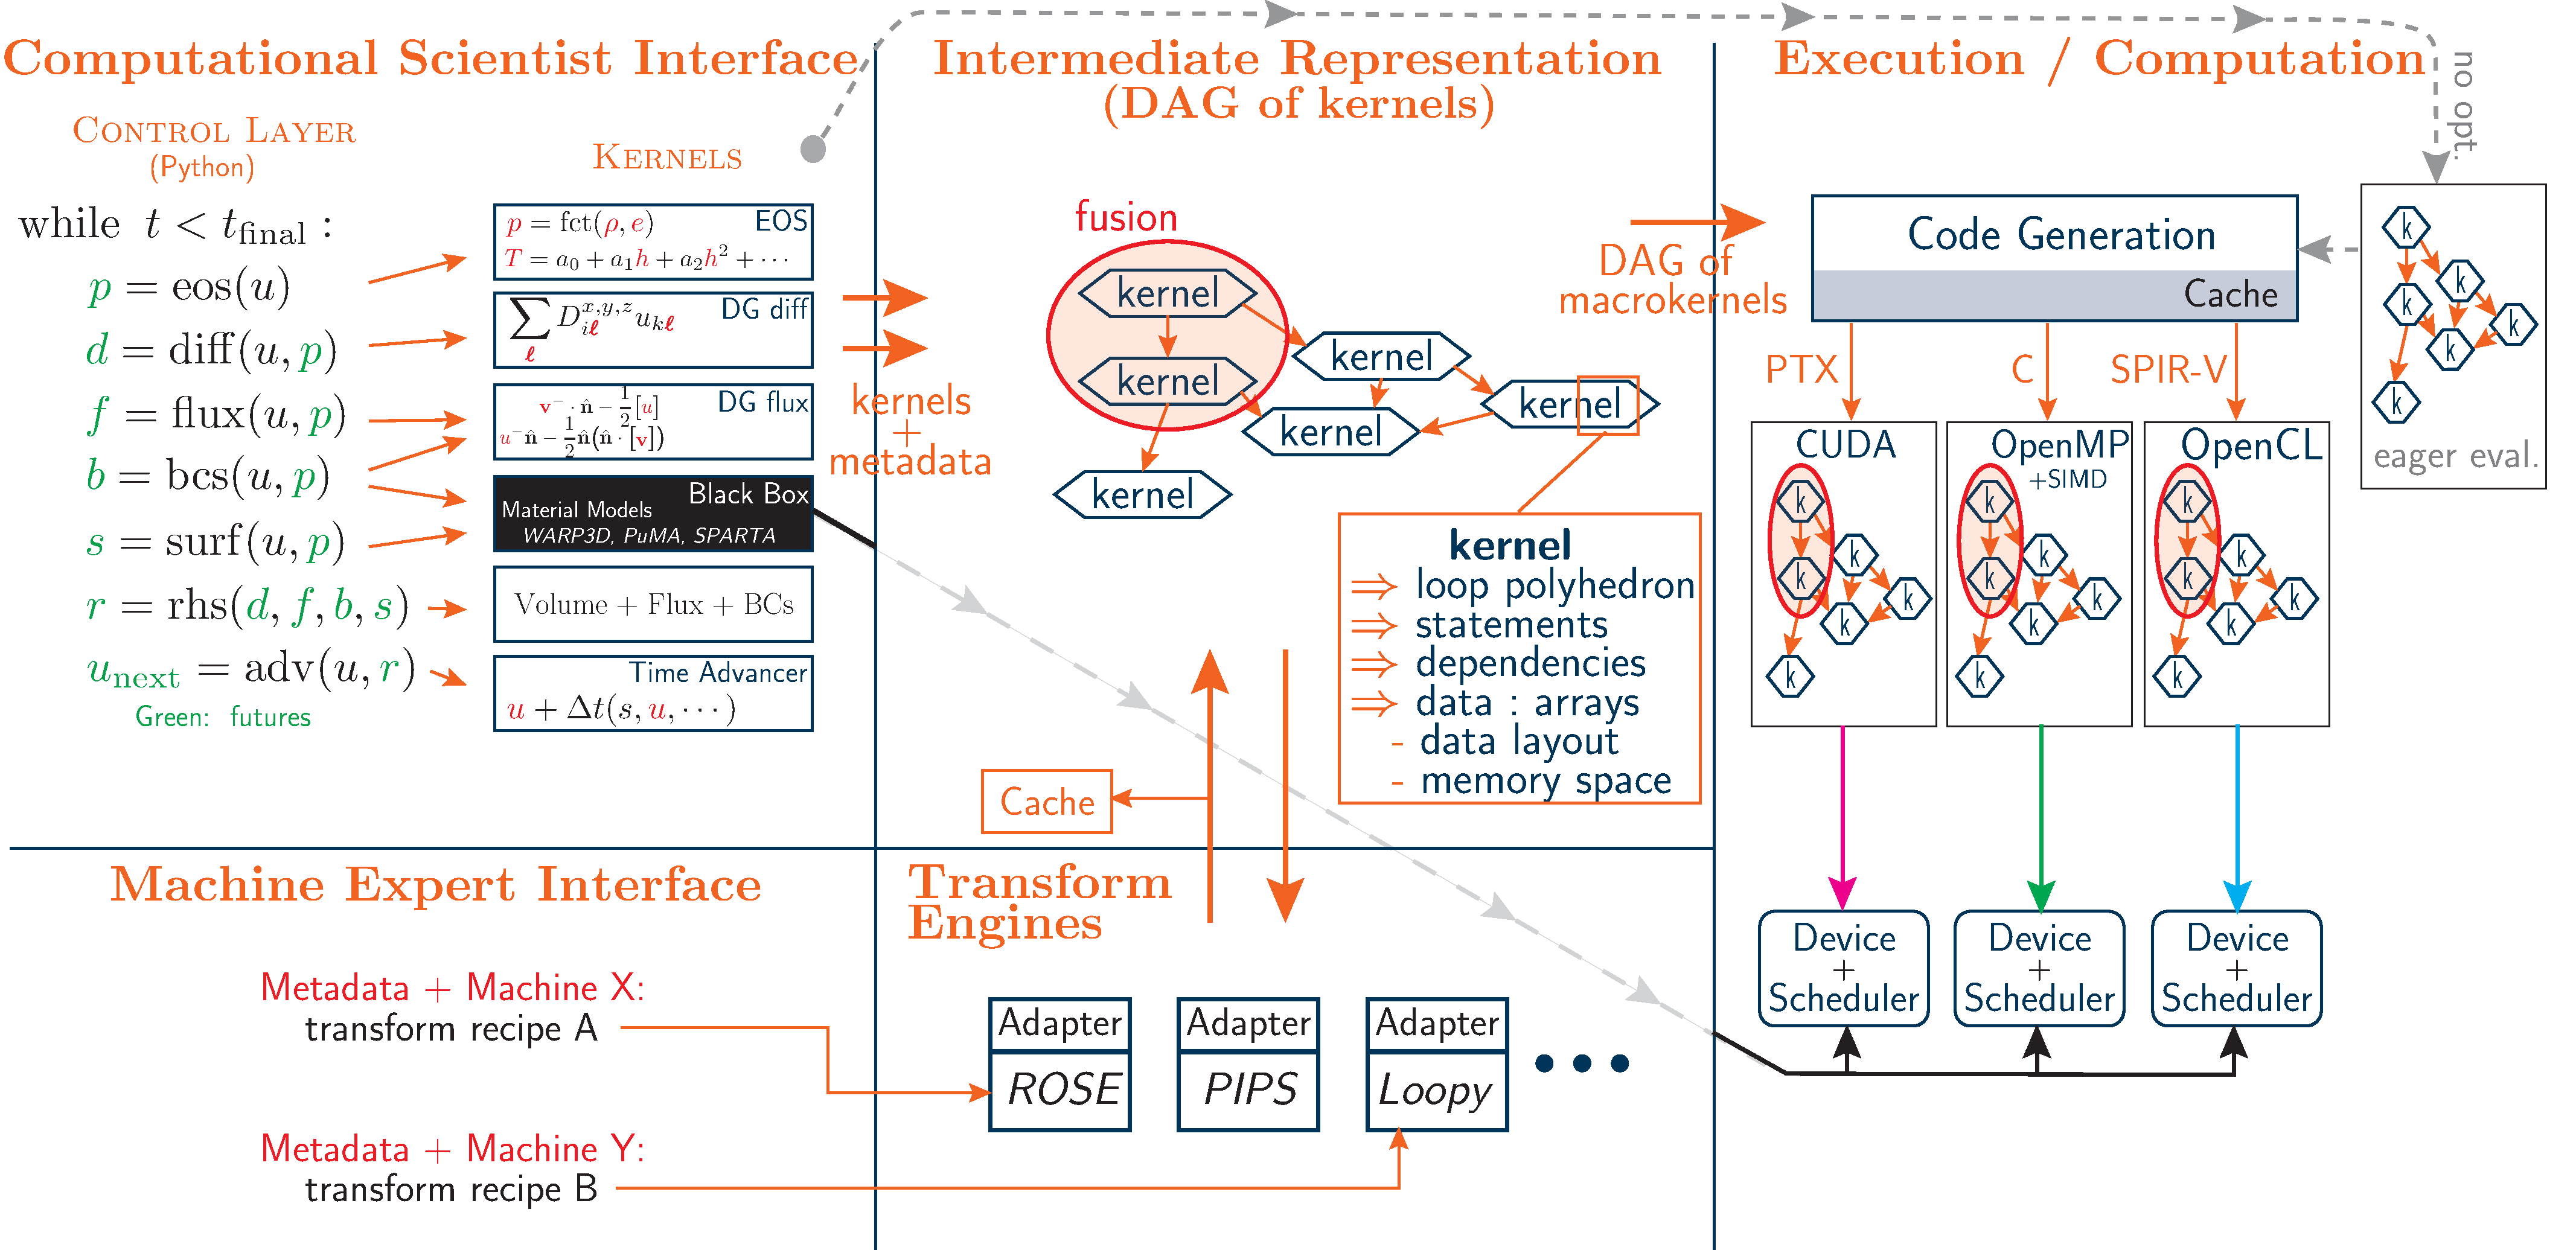
\includegraphics[width=.95\textwidth]{Figures/controllayer-new.pdf}
  % \vspace*{-5pt}
  \end{center}
\end{frame}
% Add another comment


\begin{frame}\frametitle{Simulation Infrastructure}
\begin{multicols}{2}
\begin{itemize}
\item Infrastructure provides:
  \begin{itemize}
  \item DG operators (e.g., mass, stiffness, grad, div)% , ($\mathcal{S}$)
  \item Multiple parallel discrete geometries \prj{\tiny}{M.~Smith}
   % and other machinery, spectral domain access, etc, interior\_trace\_pair - selects all interior faces
  \item Compute device access
  \item Symbolic infrastructure - great for verification
  \end{itemize}
\end{itemize}
\columnbreak
\begin{itemize}
\item \textit{MIRGE-Com} library provides:
  \begin{itemize}
  \item Conservation-law-specific data structures
  \item Simulation / driver API
  \item Prediction-relevant
    \begin{itemize}
    \item RHS operators
    \item Model-specific constructs (e.g., EOS, transport, reactions)
    \item Boundary and numerical fluxes
    \end{itemize}
  \end{itemize}
\end{itemize}
\end{multicols}
\vspace{-10pt}
\lstinputlisting[style=kkcodestyle, basicstyle=\tiny, language=Python]{Figures/mtc/rhs_sample.py}
%\begin{multicols}{2}
%  \lstinputlisting[style=kkcodestyle, basicstyle=\tiny, language=Python]{Figures/mtc/rhs_sample2.py}
%\columnbreak
%  \lstinputlisting[style=kkcodestyle, basicstyle=\tiny, language=Python]{Figures/mtc/rhs_sample3.py}
%\end{multicols}
\end{frame}

% This is my edit.

\begin{frame}\frametitle{Prediction-supporting Development}
  \begin{center}
  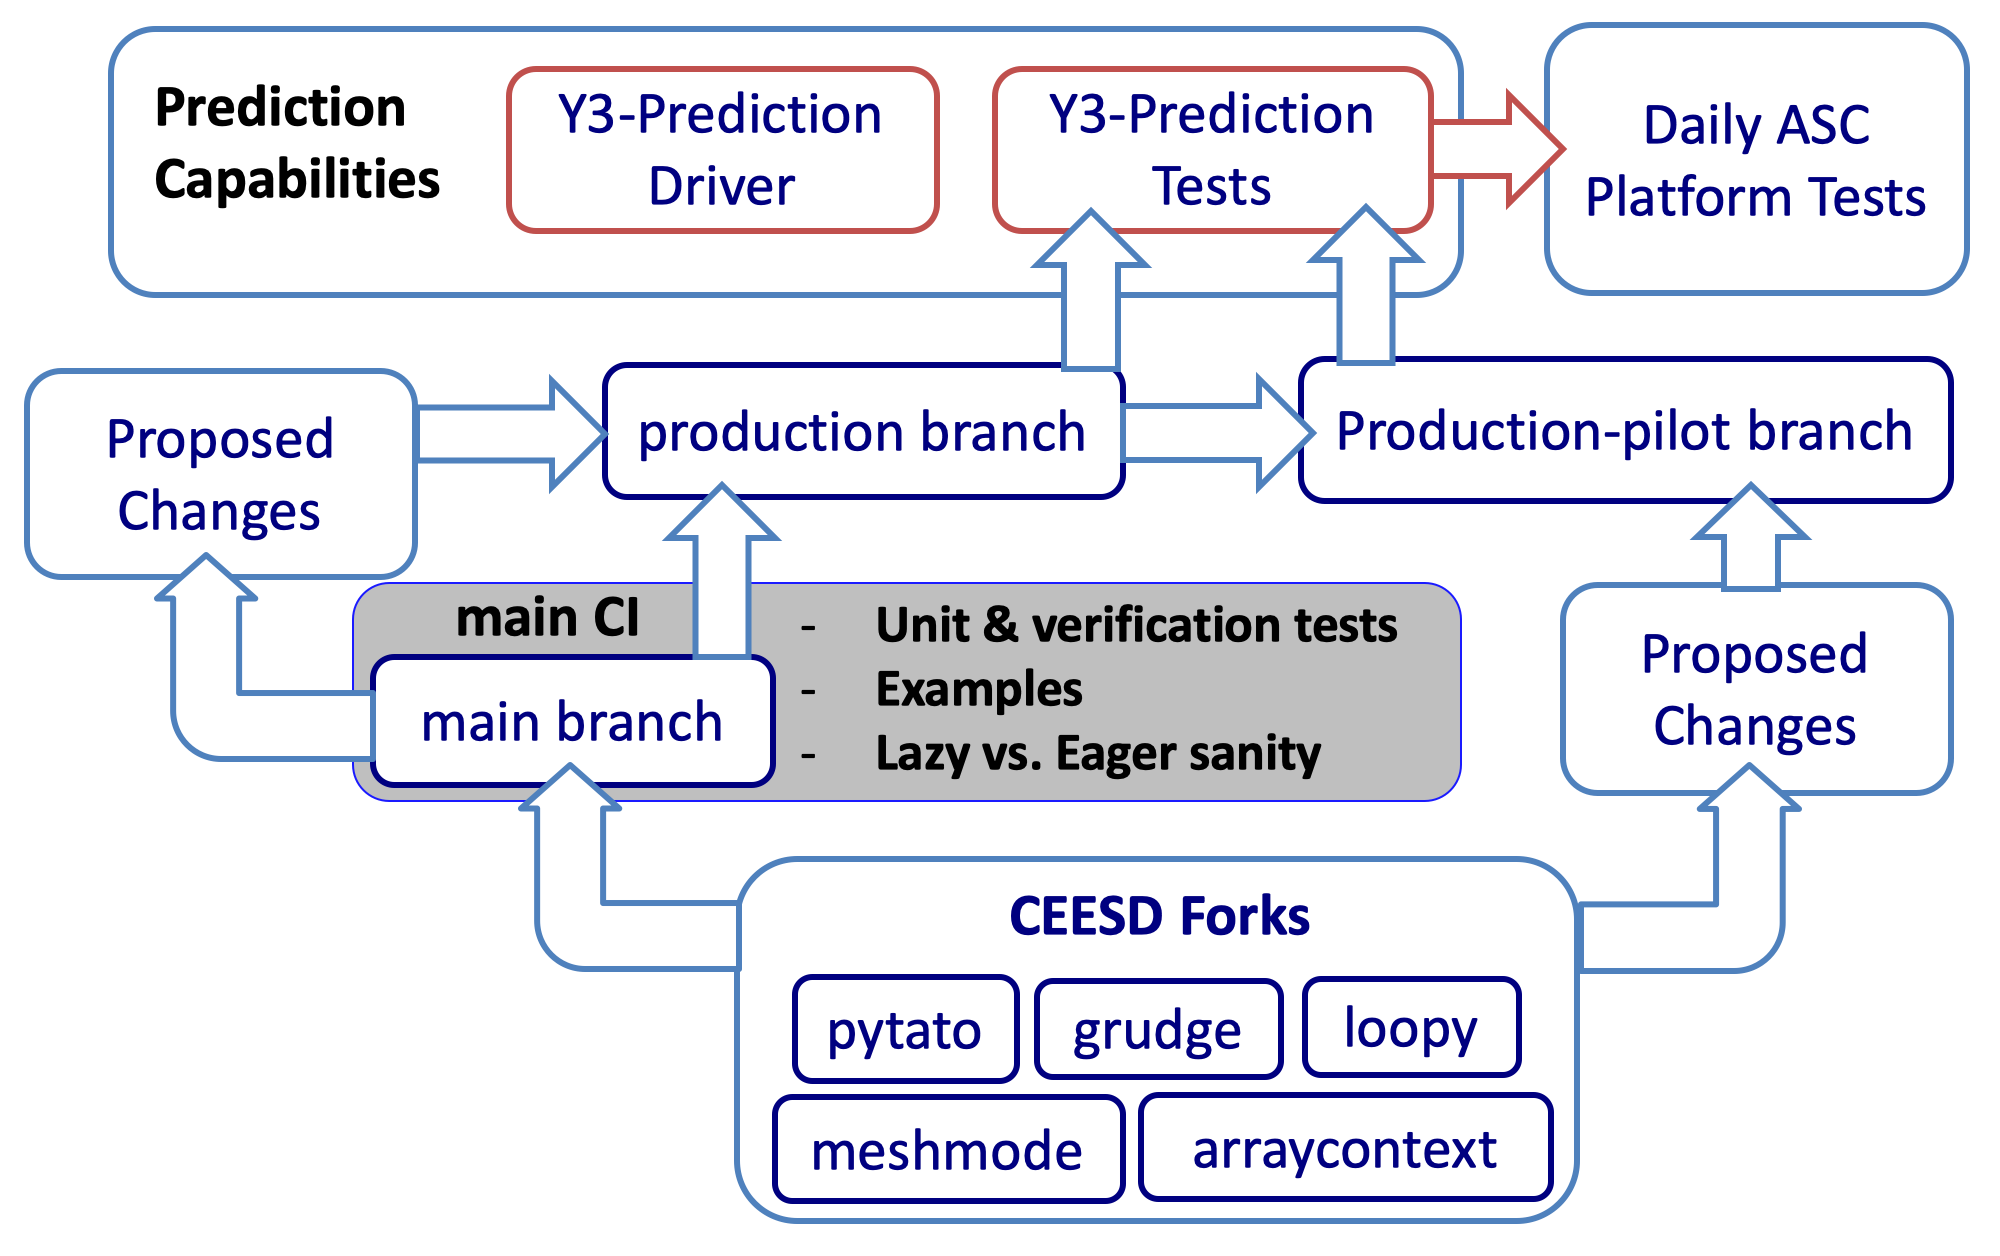
\includegraphics[width=.65\textwidth]{Figures/DevelopmentTestingFlow.png}
  \vspace*{-5pt}
  \end{center}
  \begin{center}
  % \vspace*{-15pt}
  \begin{itemize}
  \item Prediction-supporting development process
  \item Prediction-targeted testing mechanism
  \item Continuous integration and daily ASC platform testing
  \end{itemize}
  \end{center}
  \begin{tikzpicture}[remember picture, overlay]
    \node[anchor=south west, xshift=270pt, yshift=120pt] at (current page.south west) {
     
\includegraphics[width=0.03\textwidth]{Figures/github_logo.png}
    };
    \fill <2> [fill=white, opacity=0.8] (current page.south west) + (0.5,0.5) rectangle (12.5,7.5);
     \node <2> [inner sep=0pt] at (current page.center) {
     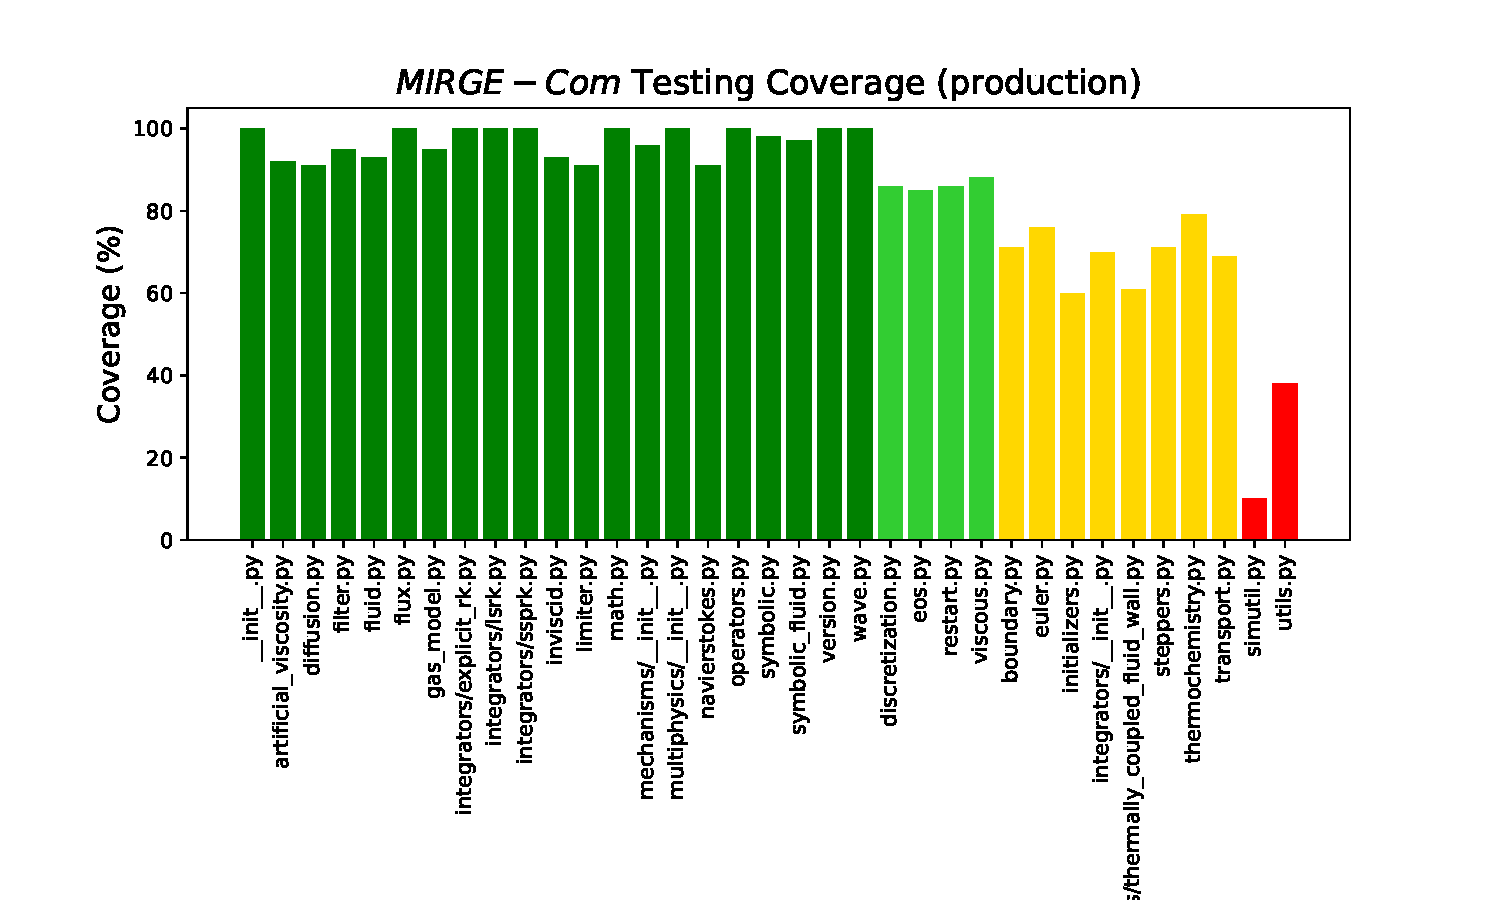
\includegraphics[width=.9\textwidth]{Figures/mtc/coverage_plot_production.pdf}
   };
  \end{tikzpicture}
\end{frame}


%\begin{frame}\frametitle{Prediction-supporting Development}
%  \begin{center}
%  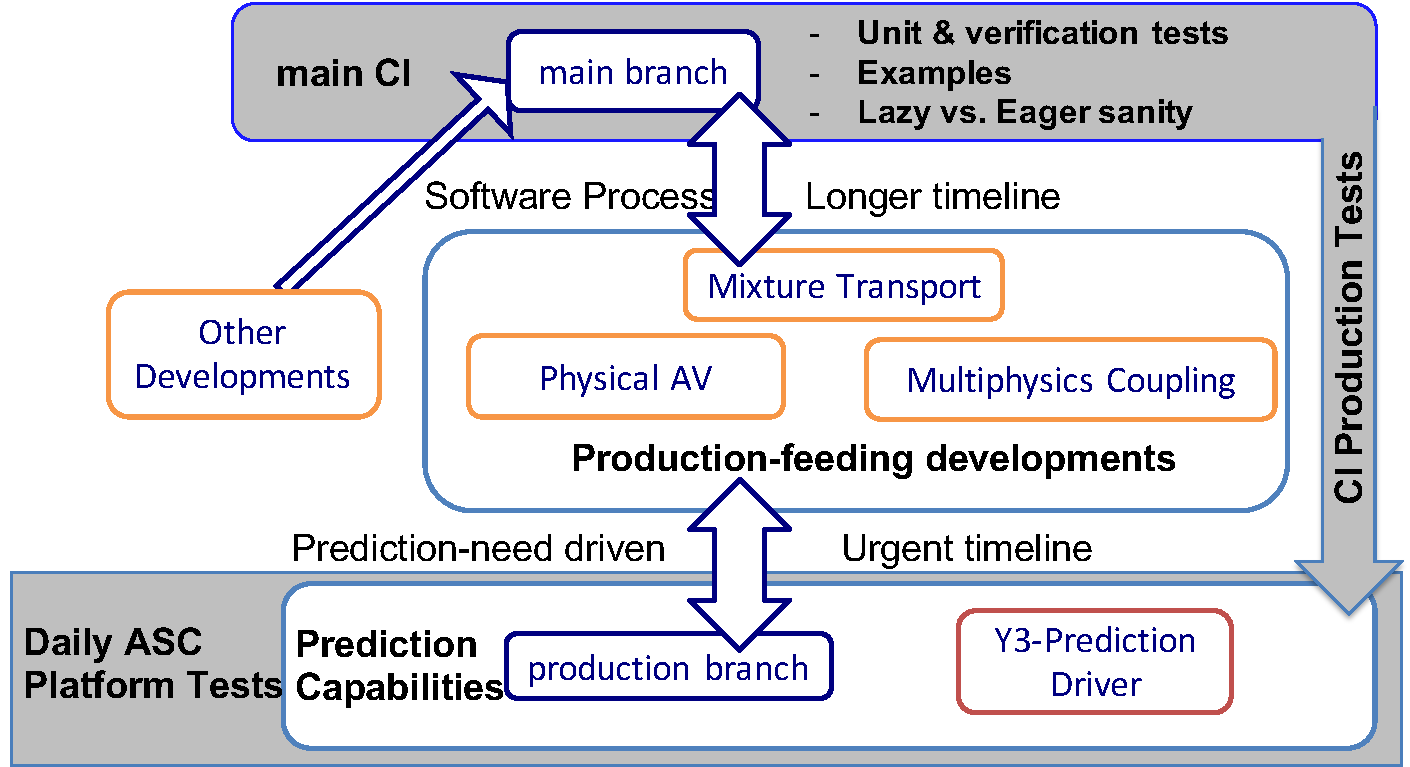
\includegraphics[width=.65\textwidth]{Figures/mtc/PredictionSupportinDevel3.pdf}
%  \vspace*{-5pt}
%  \end{center}
%  \begin{center}
%  % \vspace*{-15pt}
%  \begin{itemize}
%  \item Prediction-supporting development process
%  \item Prediction-targeted testing mechanism
%  \item Continuous integration and daily ASC platform testing
%  \end{itemize}
%  \end{center}
%  \begin{tikzpicture}[remember picture, overlay]
%    \fill <2> [fill=white, opacity=0.8] (current page.south west) + (0.5,0.5) rectangle (12.5,7.5);
%    \node <2> [inner sep=0pt] at (current page.center) {
%      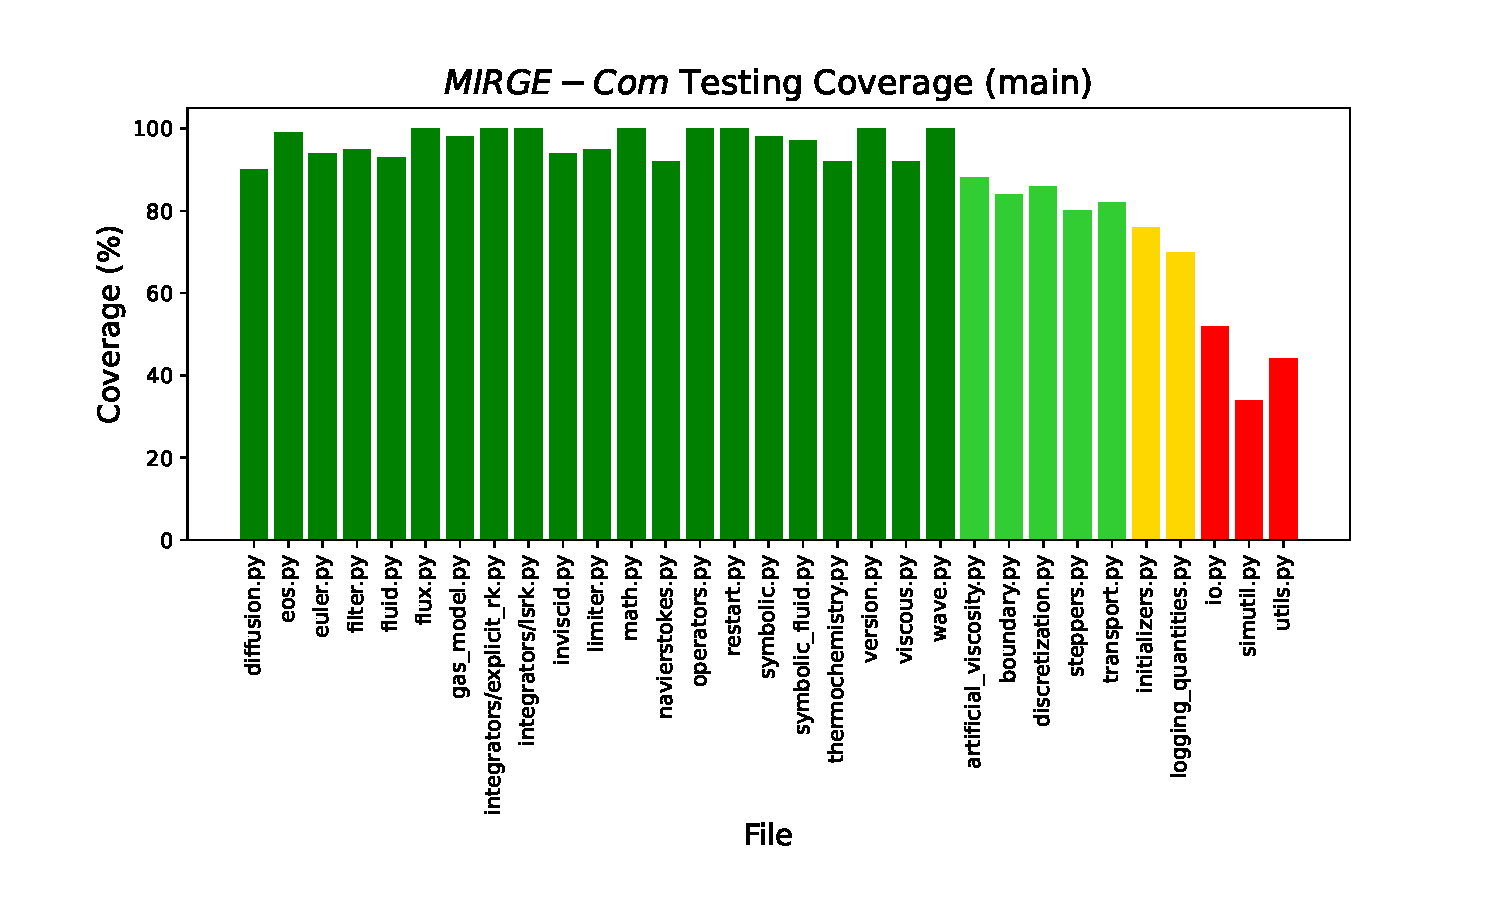
\includegraphics[width=.9\textwidth]{Figures/mtc/coverage_plot_main.pdf}
%    };
%  \end{tikzpicture}
%\end{frame}

%\begin{frame}\frametitle{Prediction-supporting Development}
%  \begin{center}
%  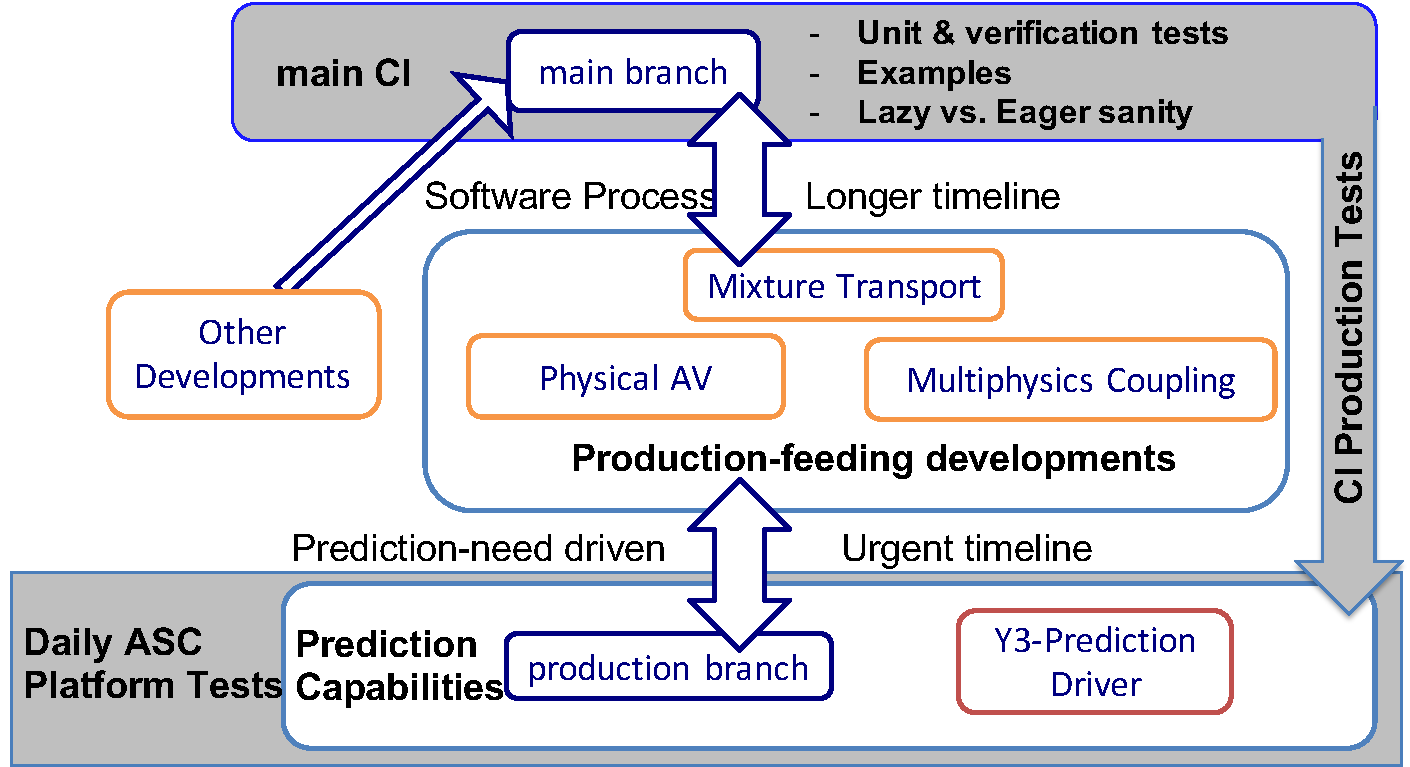
\includegraphics[width=.65\textwidth]{Figures/mtc/PredictionSupportinDevel3.pdf}
%  \vspace*{-5pt}
%  \end{center}
%  \begin{center}
%  % \vspace*{-15pt}
%  \begin{itemize}
%  \item Prediction-supporting development process
%  \item Prediction-targeted testing mechanism
%  \item Continuous integration and daily ASC platform testing
%  \end{itemize}
%  \end{center}
%\end{frame}

%\begin{frame}\frametitle{Thermochemistry Verification in \mirgecom}
%\begin{center}
% Autoignition co-verification
%\end{center}
%\begin{itemize}
%   \item Ethylene/air mixture $(1500\mathtt{K}, \rho=\mathtt{const})$
%   \item \pyrometheus-predicted profiles match \textit{Cantera}
%   \item \pyrometheus{} with implicit time integration with \textit{CVODE}
%   \item \mirgecom{} with RK4, inviscid, quiescent
%\end{itemize}
%\begin{multicols}{2}
%    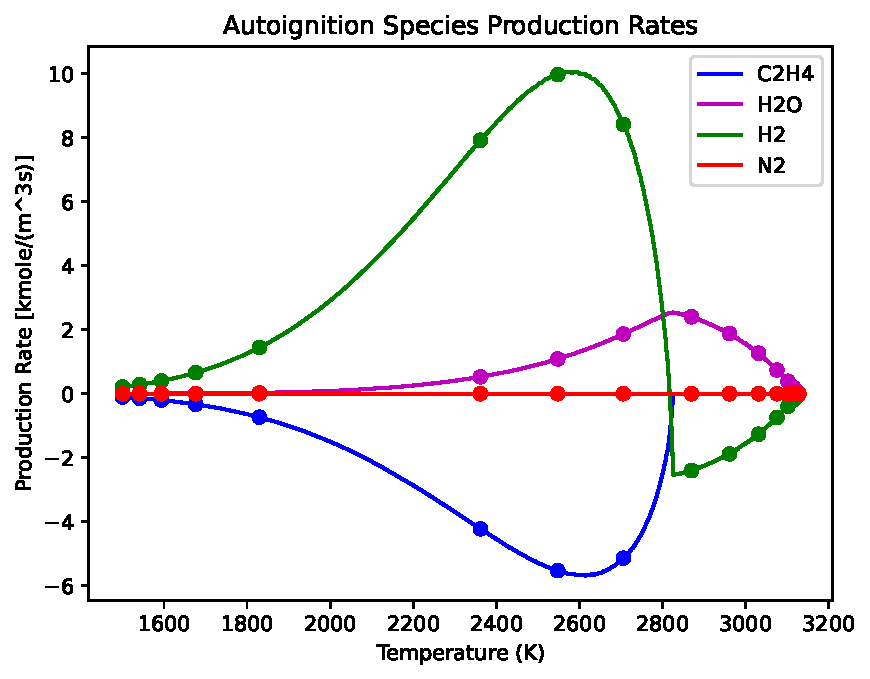
\includegraphics[width=.4\textwidth]{Figures/mtc/autoignition_rates.pdf}\\
%    \columnbreak
%    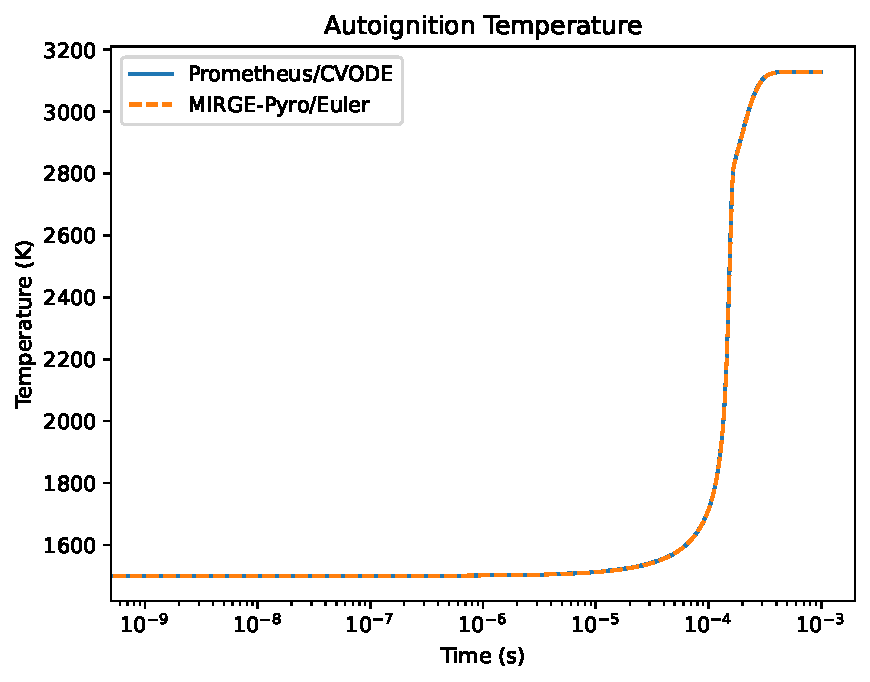
\includegraphics[width=.4\textwidth]{Figures/mtc/autoignition_temperature.pdf}
%  \end{multicols}
%\end{frame}

\begin{frame}
    \centering
    \Large
    \textbf{Performance \& Scalability}
    % Fundamentals
    % \begin{itemize}
    %    \item Strong Scaling: Fixed problem size, scaling resource
    %    \item Weak Scaling: Scaled problem size, fixed work/resource
    %    \item Versatility: Portability, resource options
    %\end{itemize}
    % MIRGE-Com scaling in Y3
    % \item \textbf{MIRGE-Com Scaling in Y3}
    % \begin{itemize}
    %    \item Why do we care?  (Enabling prediction!)
    %    \item Performance Snapshots
    %    \begin{itemize}
    %        \item Weak Scaling Achievements
    %        \item Strong Scaling Insights
    %        \item Lassen Monitoring Highlights
    %    \end{itemize}
    % Why do we care about scalability?
    % Current snapshot
    % Scalability datasets
    % Timings on Lassen
\end{frame}

\begin{frame}\frametitle{Performance \& Scalability}
\begin{itemize}
%\item What performance?
%\begin{itemize}
\item Computational performance: Speed or FLOPS
% VS. the machine itself, vs. expectation
\item Parallel performance: Scalability or efficiency
\begin{itemize}
\item Strong scaling: Fixed problem size, scaling resources
\item Weak scaling: Fixed work/resource, scaling problem size with resource
\item Mesh scaling: Scaling work, fixed resource
\end{itemize}
\item I/O and memory performance: Bandwidth, bytes/second
\item Cost performance
\begin{itemize}
\item Energy efficiency
\item Total time to solution (TTS)
\item FLOPS/Fidelity
\item Usability/Productivity
\end{itemize}
\item Why should we care about scalability? (enables prediction!)
\begin{itemize}
\item Weak scaling out to prediction-scale
\item Versatility, portability, and resource options
\end{itemize}
\end{itemize}
\end{frame}

\begin{frame}\frametitle{Performance \& Scalability}
\begin{minipage}[t][0.4\textheight][t]{\textwidth}
\begin{center}
New: prediction-enabling performance
\end{center}
\begin{multicols}{2}
\begin{itemize}
\item Scaling as expected (mostly)
\item Small problems are expensive
\columnbreak
\item OOM: SVM/Unified memory % \prj\tiny{07c, M.~Diener}
\item Mem growth: Garbage collection
\end{itemize}
%\item Absolute performance could be better
%\item Recent focus: memory growth
%\end{itemize}
\end{multicols}
\end{minipage}\vfill
\vspace{-20pt}
\begin{minipage}[t][0.4\textheight][t]{\textwidth}
\centering
%Grid Scaling\\
%\end{center}
%\begin{center}
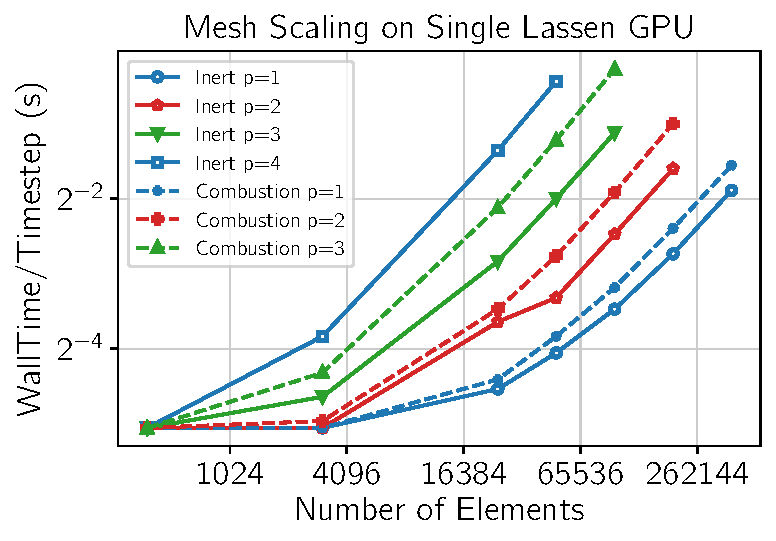
\includegraphics[width=.4\textwidth]{Figures/mtc/combozzle_gridscale.pdf}\hspace{30pt}
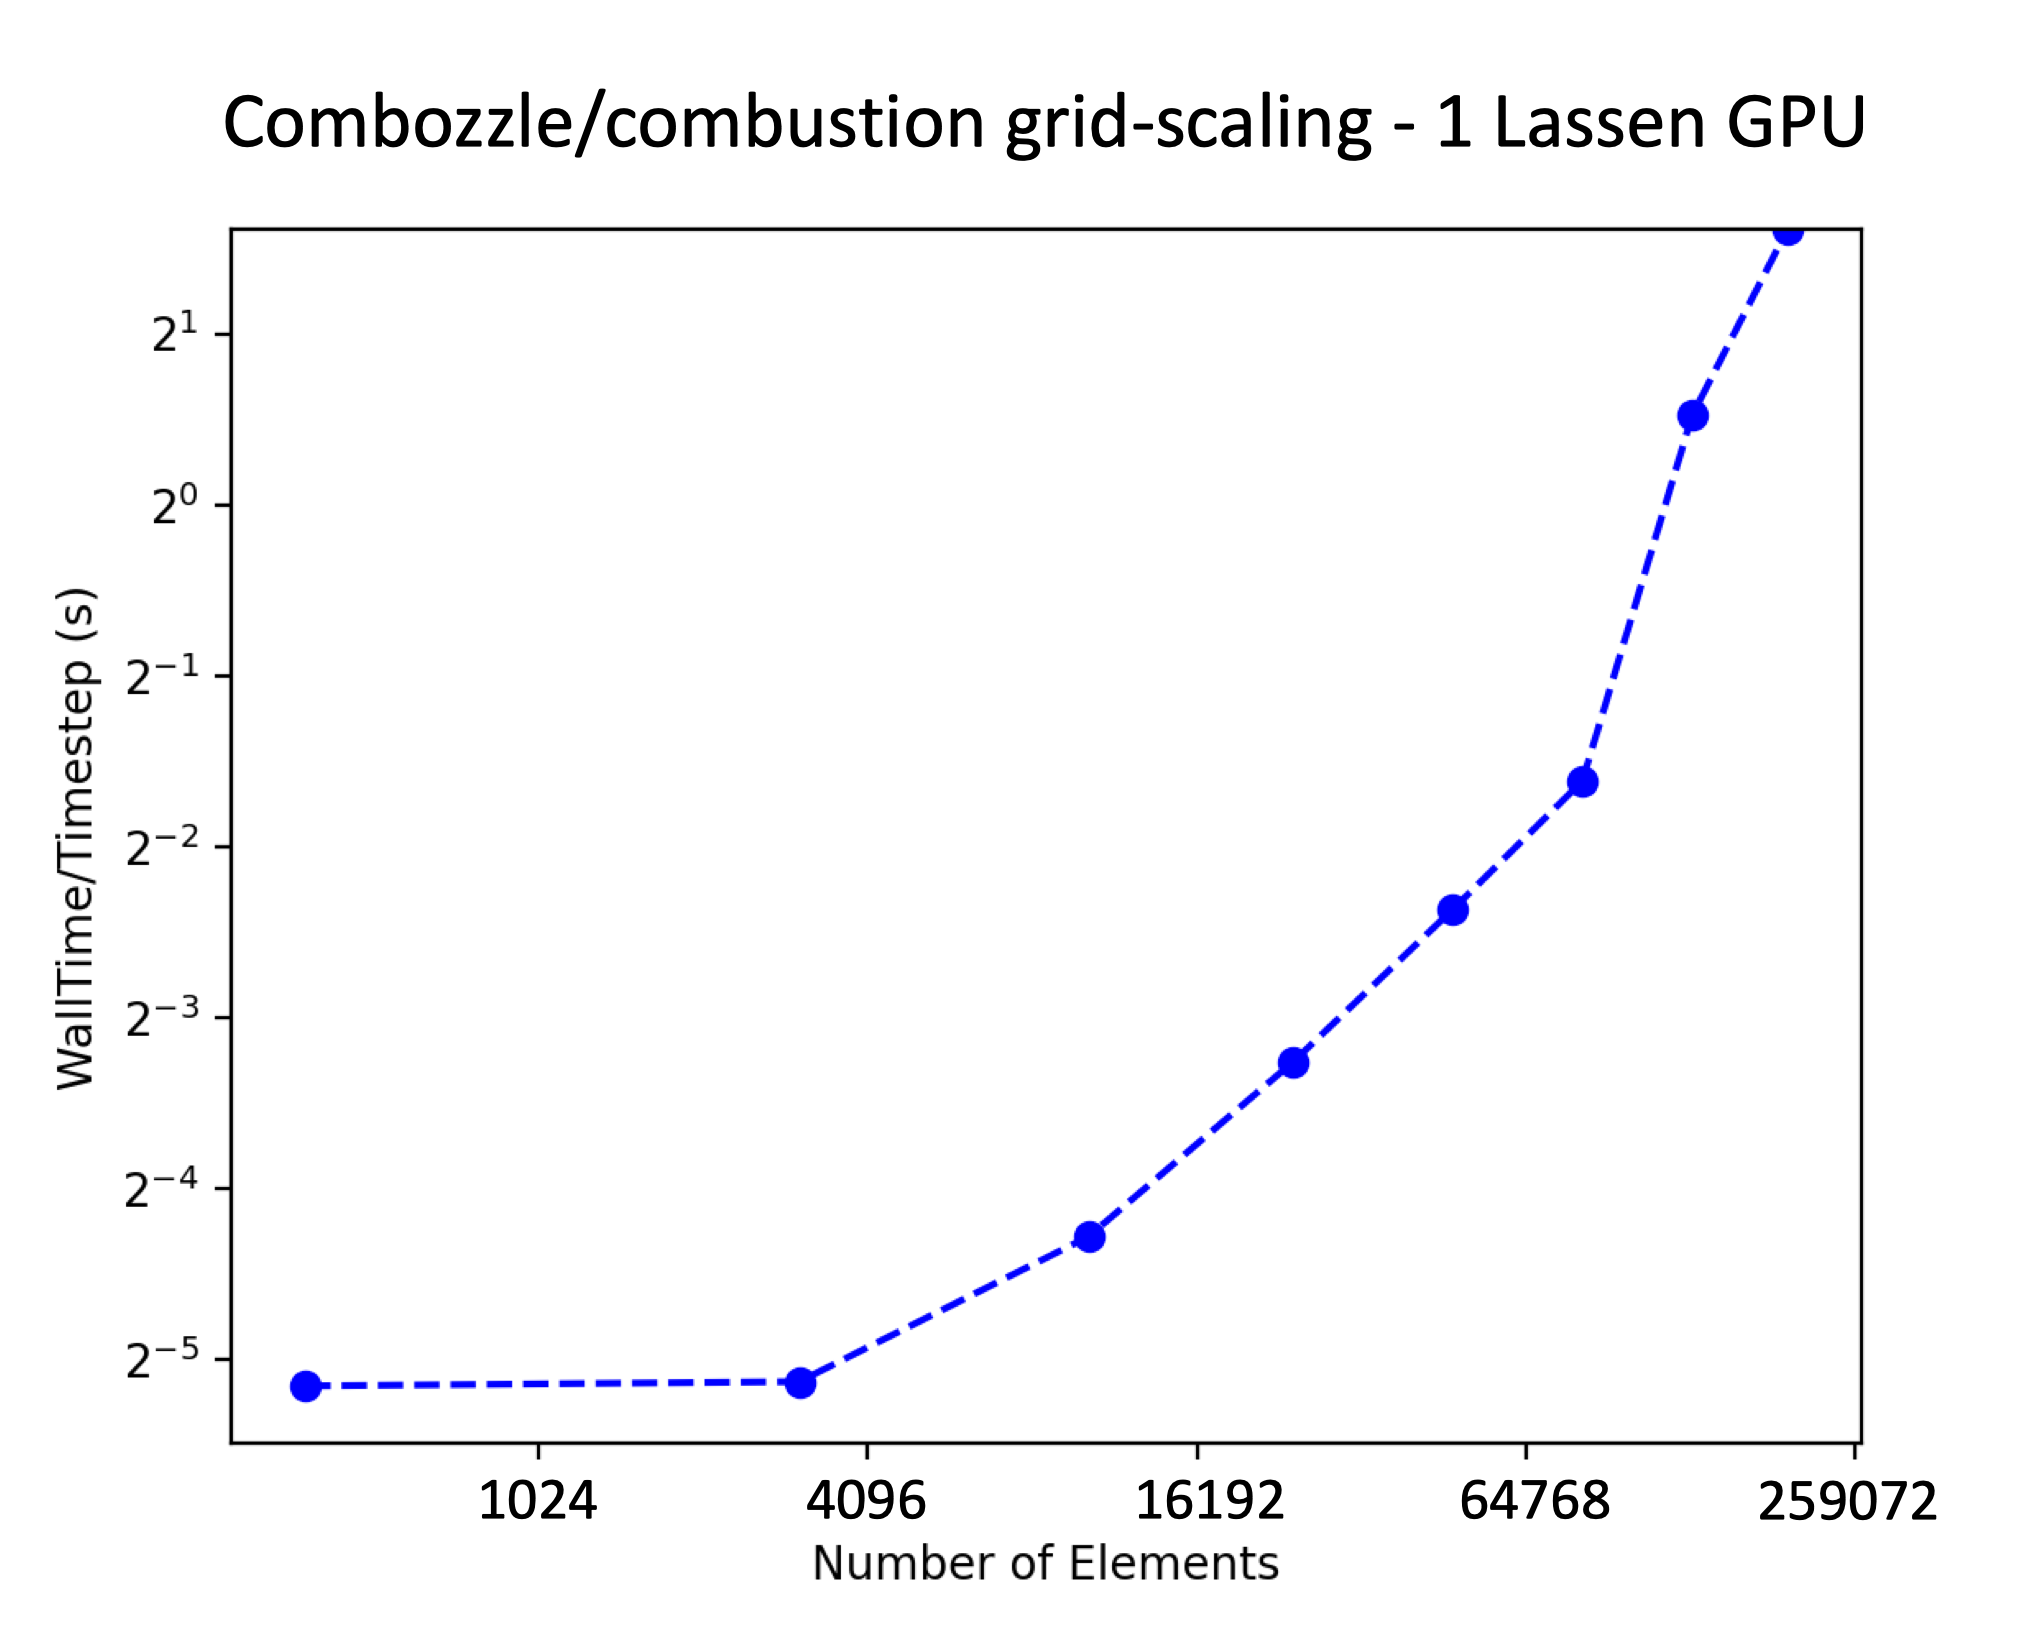
\includegraphics[width=.4\textwidth]{Figures/mtc/comboz_gridscale_svm.png}
\end{minipage}
\end{frame}


\begin{frame}\frametitle{DAG Splat Effect}
\begin{minipage}[t][0.4\textheight][t]{\textwidth}
\begin{center}
New: prediction-enabling performance
\end{center}
\begin{multicols}{2}
\begin{itemize}
\item DAG Splat: DAG for each boundary
\item Limits weak scaling - DAG for each neighbor
\columnbreak
\item Mitigation: Metis $\to$ 1D decomp
\item Real fix: Function calls in the DAG (aka function outlining)
\end{itemize}
\end{multicols}
\end{minipage}\vfill
\vspace{-20pt}
\begin{minipage}[t][0.4\textheight][t]{\textwidth}
\centering
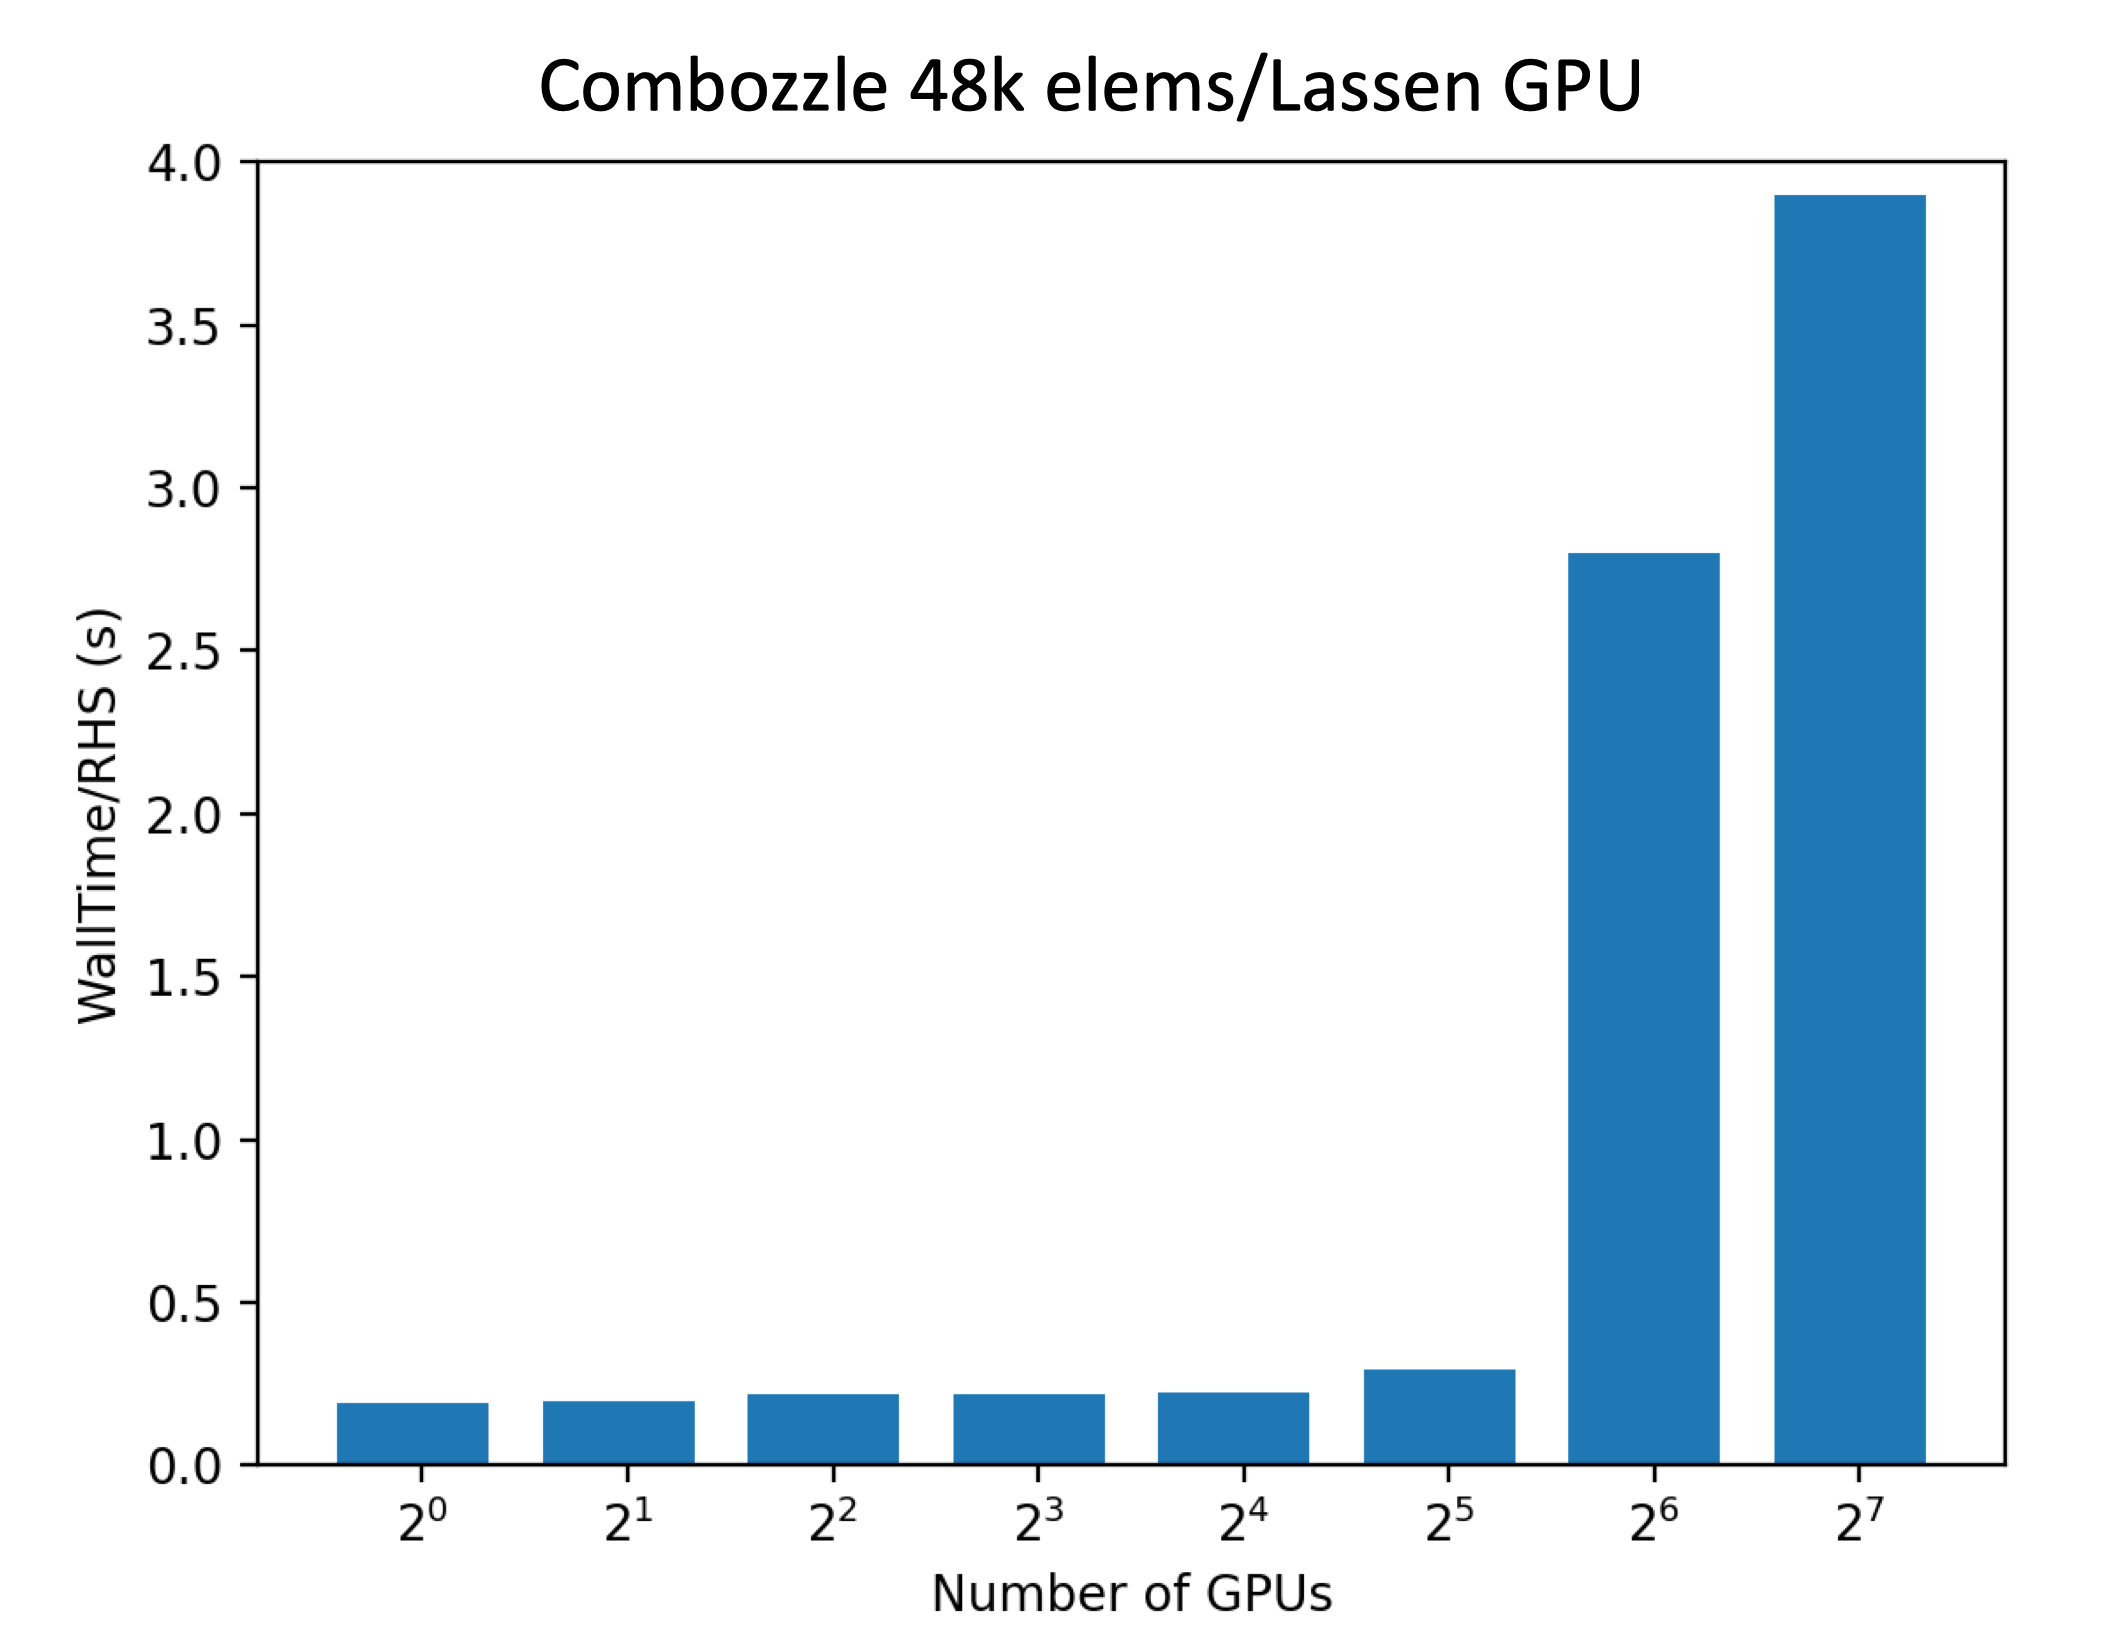
\includegraphics[width=.4\textwidth]{Figures/mtc/combozzle_weak_bad_partitioning.png}\hspace{30pt}
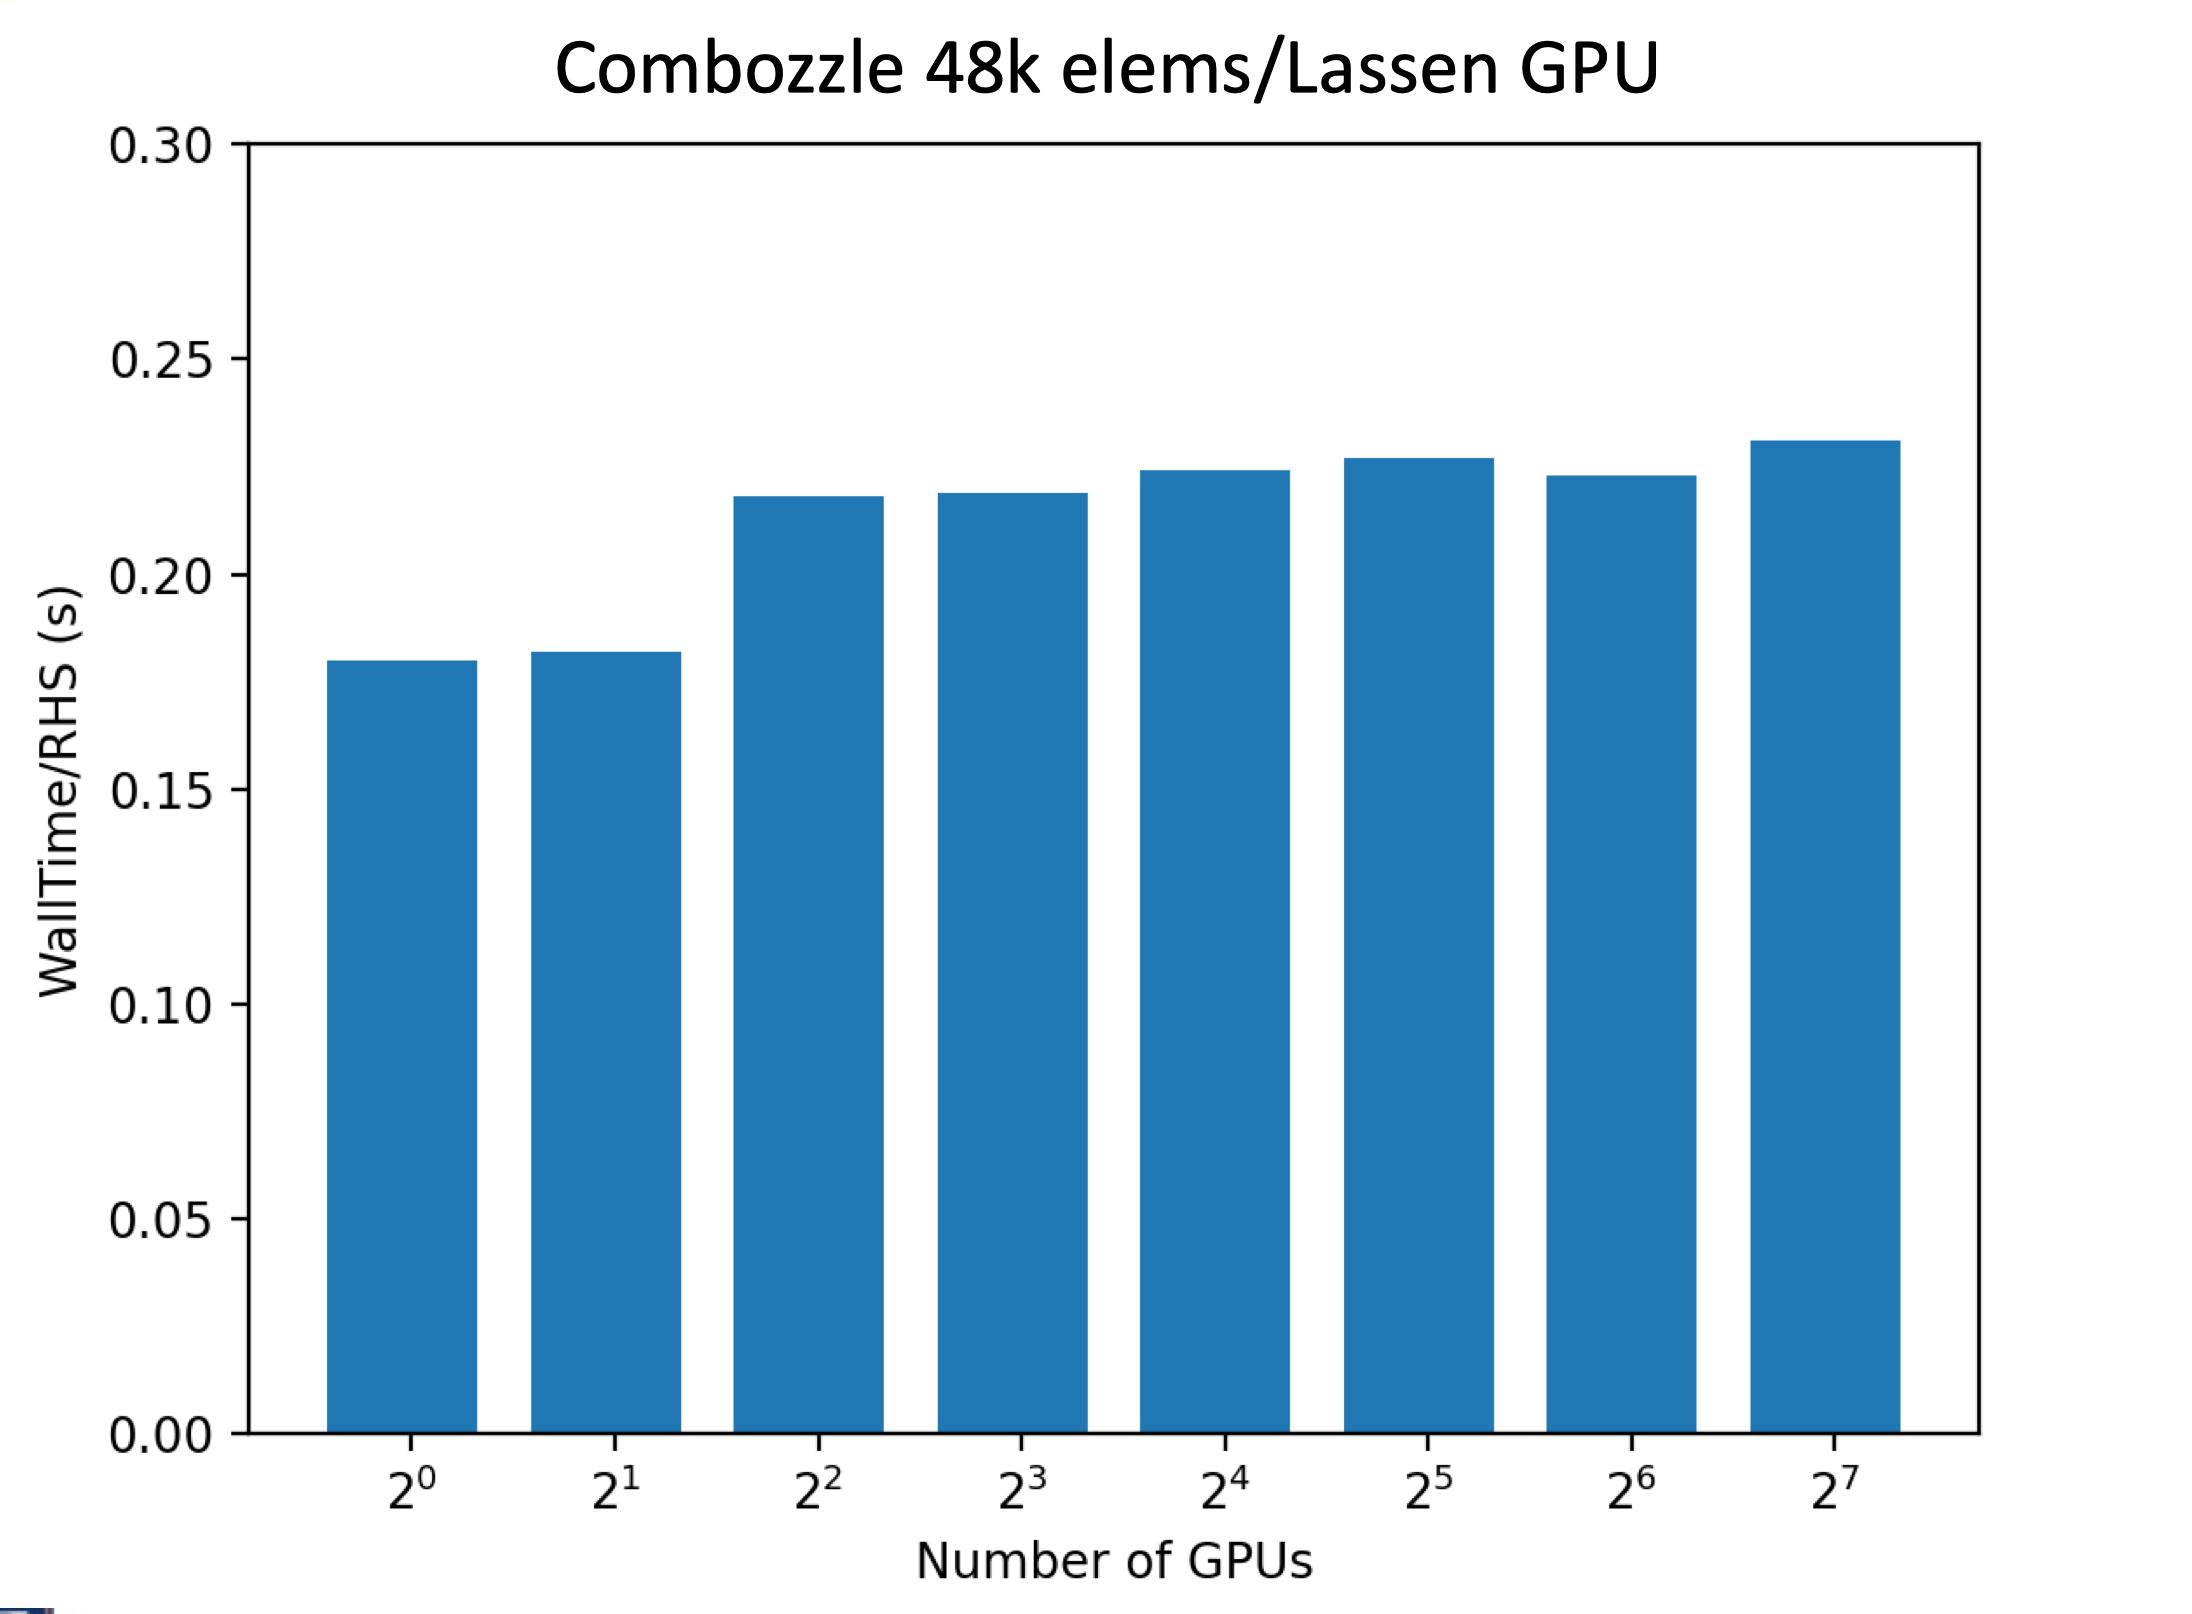
\includegraphics[width=.4\textwidth]{Figures/mtc/combozzle_weak_sliced_partitioning.png}
\end{minipage}
\end{frame}

\begin{frame}\frametitle{DAG Splat Mitigation}
\begin{minipage}[t][0.4\textheight][t]{\textwidth}
\begin{center}
New: prediction-enabling performance
\end{center}
\begin{multicols}{2}
\begin{itemize}
\item DAG Splat: DAG for each boundary
\item Limits weak scaling - DAG for each neighbor
\columnbreak
\item Mitigation: Metis $\to$ 1D decomp
\item Real fix: Function calls in the DAG (a.k.a. outlining)   %\prj\tiny{Kaushik Kulkarni}
\end{itemize}
\end{multicols}
\end{minipage}\vfill
%\vspace{-100pt}
\begin{minipage}[t][0.4\textheight][t]{\textwidth}
\centering
%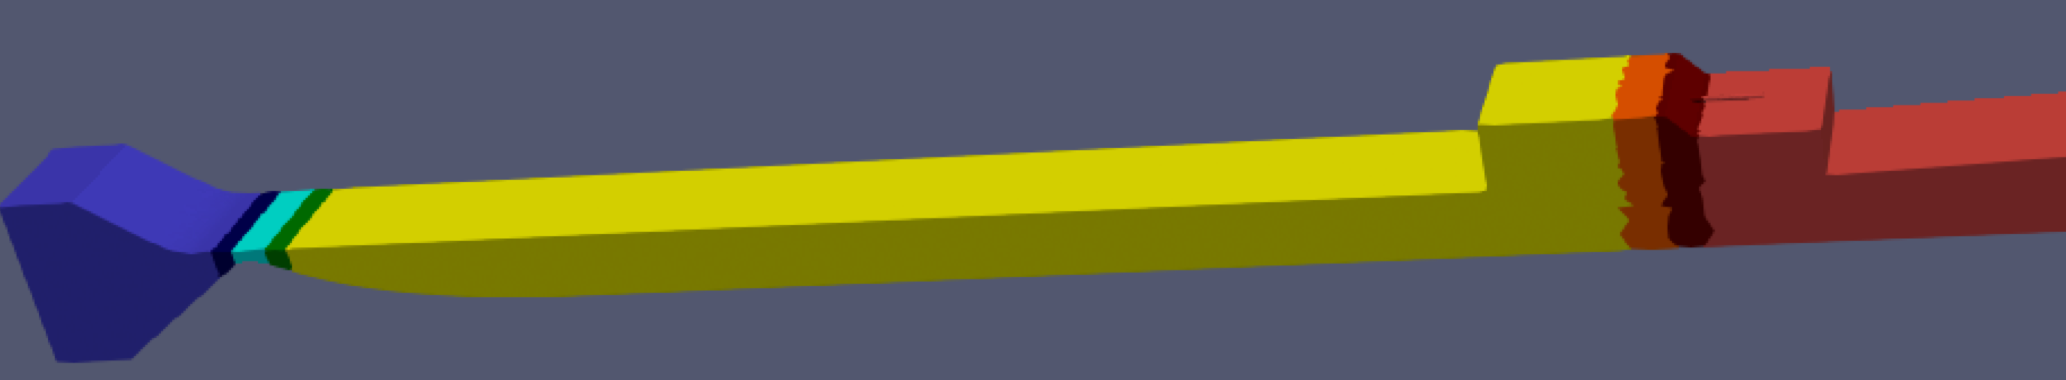
\includegraphics[width=.9\textwidth]{Figures/mtc/1dpart_bal.png}\\
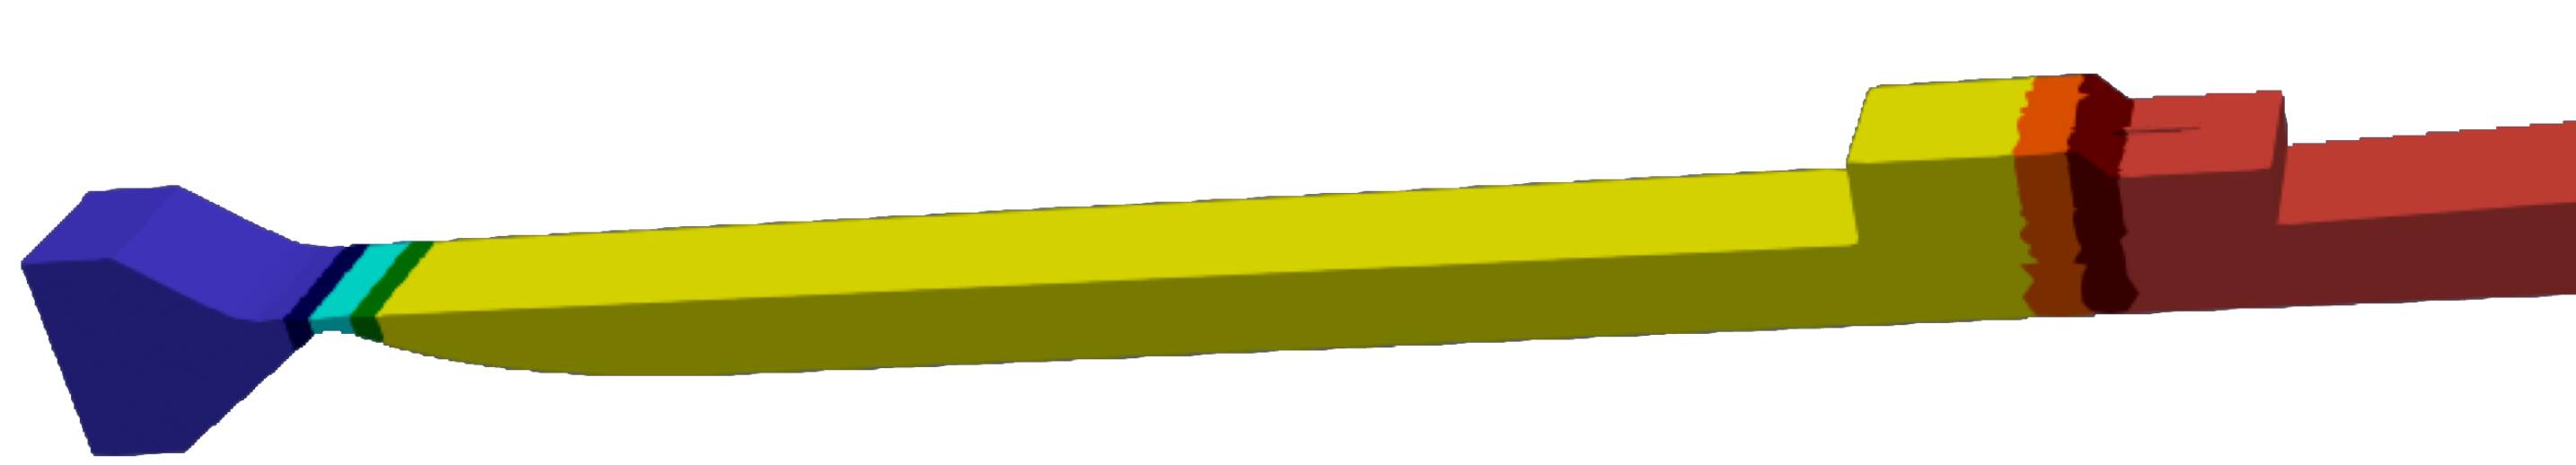
\includegraphics[width=.9\textwidth]{Figures/mtc/1dpartshiny.png}\\
%\vspace{-50pt}
\begin{center}
Y2 Domain Decomposition
\end{center}
\end{minipage}
\end{frame}

\begin{frame}\frametitle{Scaling with 1D Partitioning}
\begin{minipage}[t][0.4\textheight][t]{\textwidth}
\begin{center}
New: prediction-enabling performance
\end{center}
\begin{multicols}{2}
\begin{itemize}
\item DAG Splat: DAG for each boundary
\item Limits weak scaling - DAG for each neighbor
\columnbreak
\item Mitigation: Metis vs. 1D decomp
\item Real fix: Function calls in the DAG (a.k.a. outlining)  \prj\tiny{M.~Smith}% \prj\tiny{Kaushik Kulkarni}
\end{itemize}
\end{multicols}
\end{minipage}\vfill
\vspace{-20pt}
\begin{minipage}[t][0.4\textheight][t]{\textwidth}
\centering
%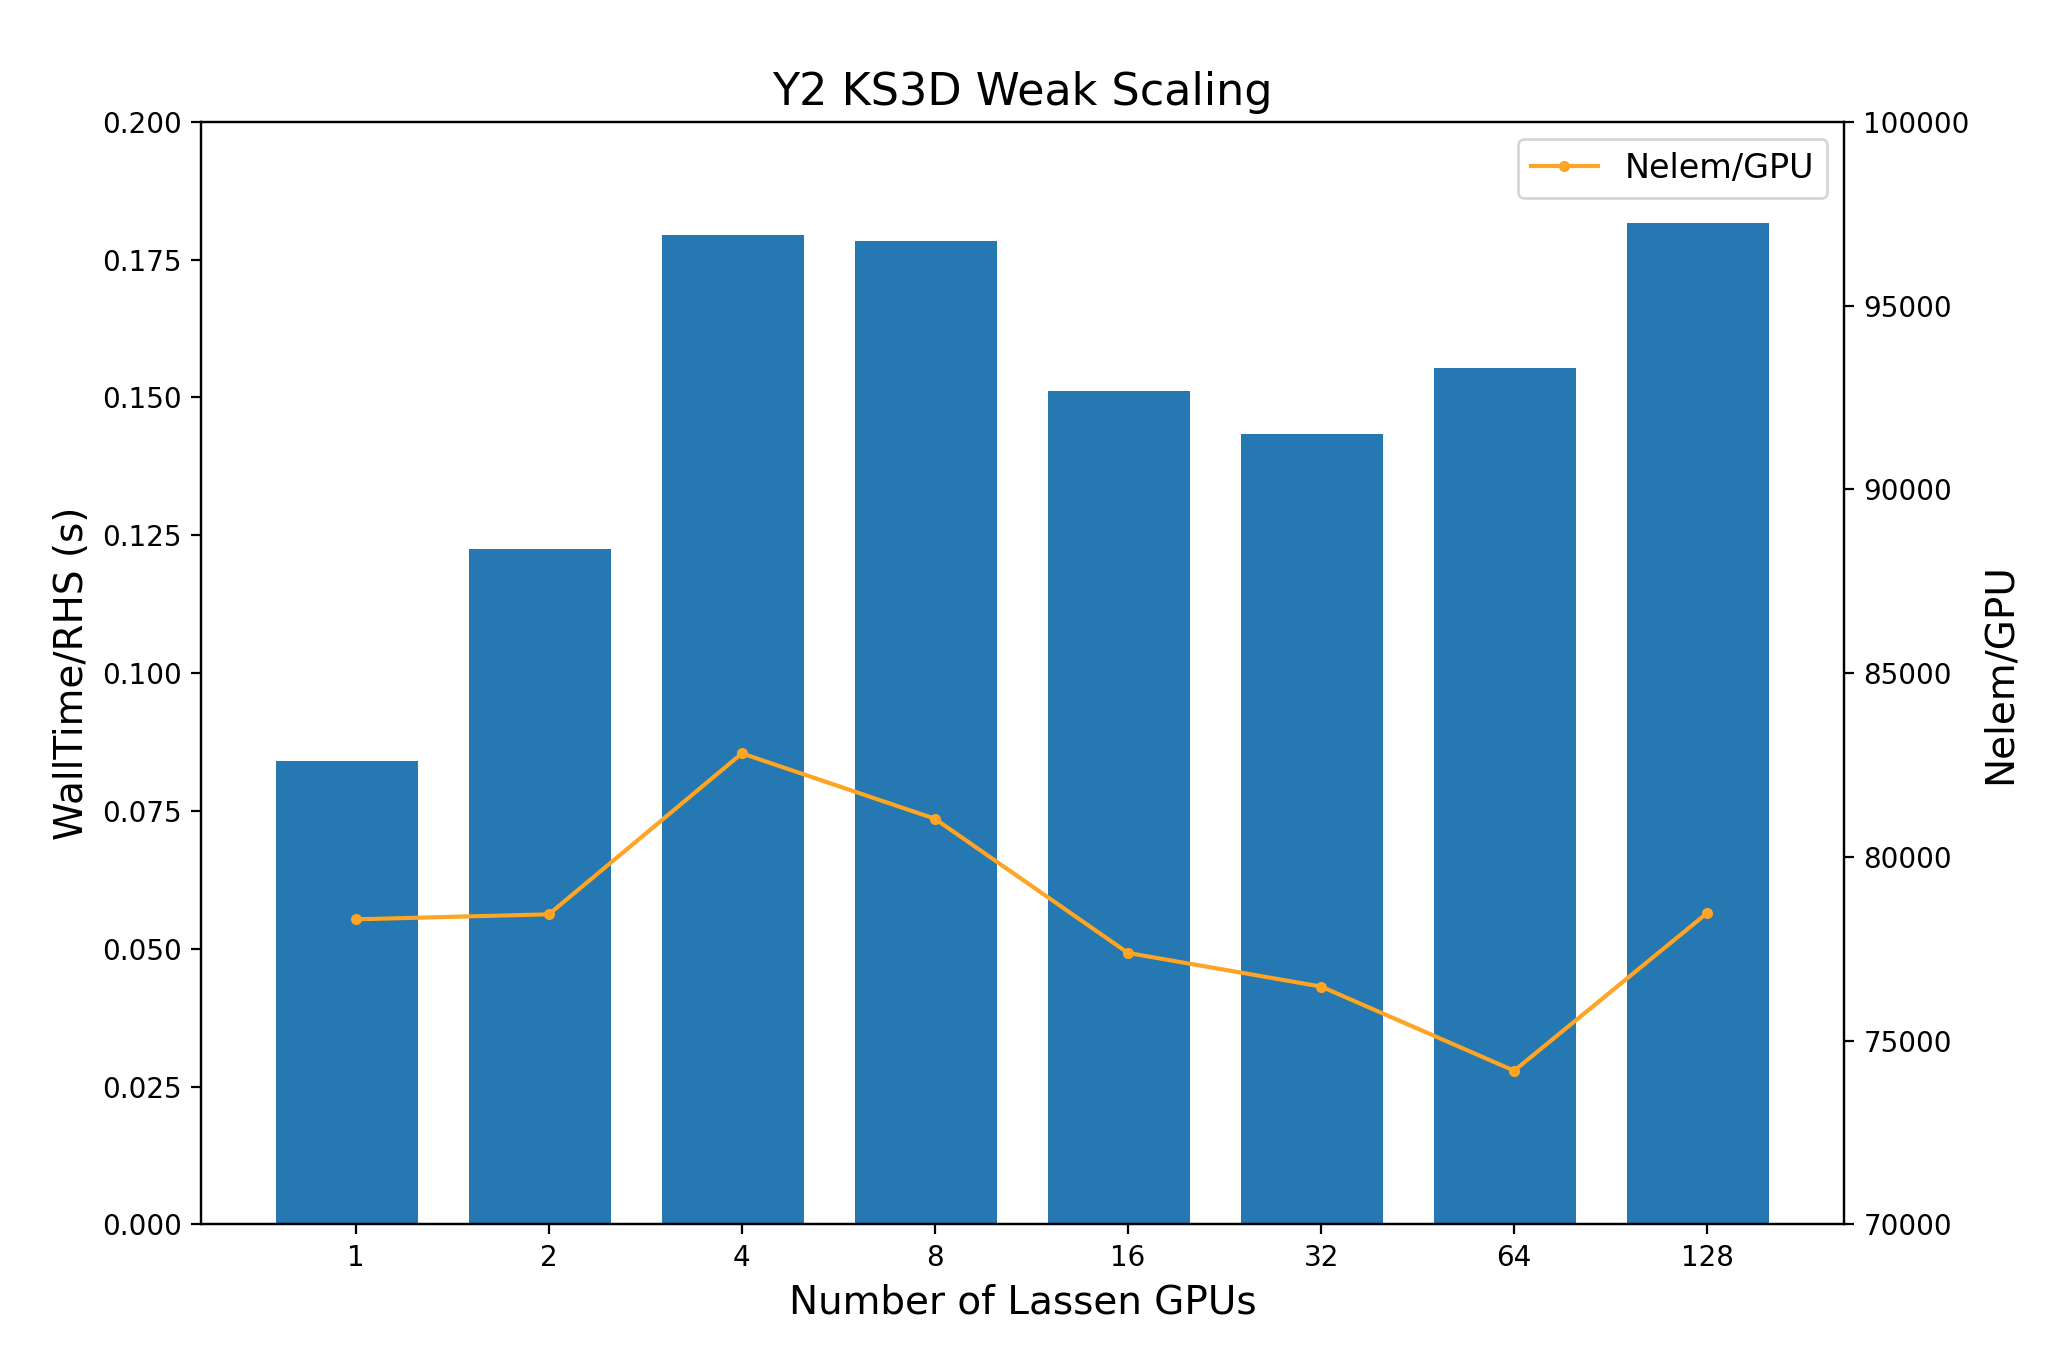
\includegraphics[width=.48\textwidth]{Figures/mtc/y2ks3d_weak.png}
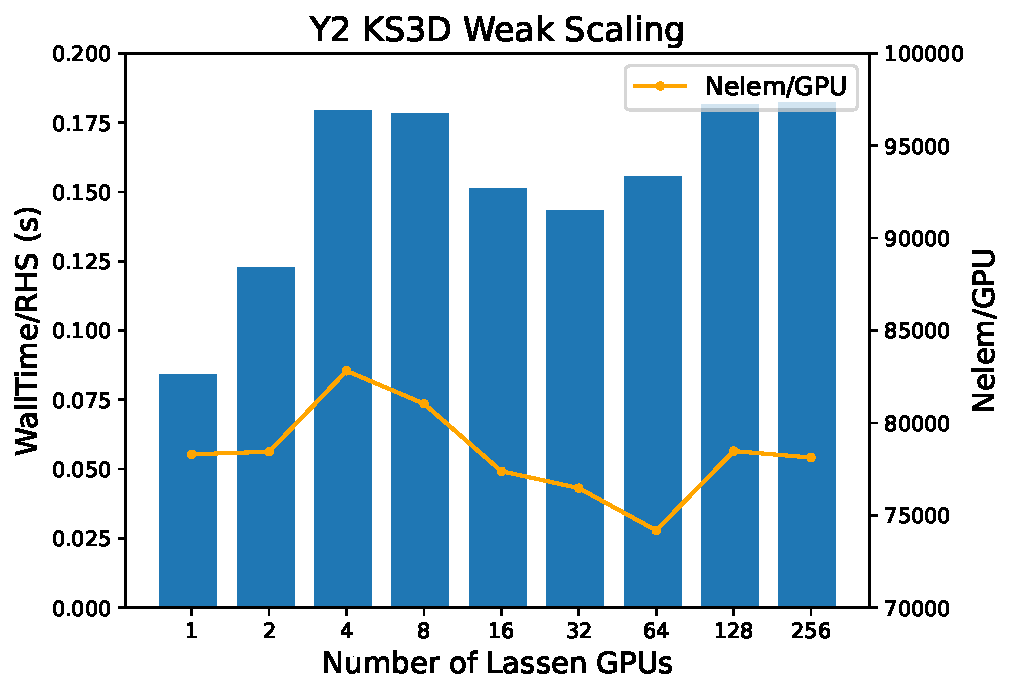
\includegraphics[width=.48\textwidth]{Figures/mtc/y2-prediction_weak_scaling.pdf}
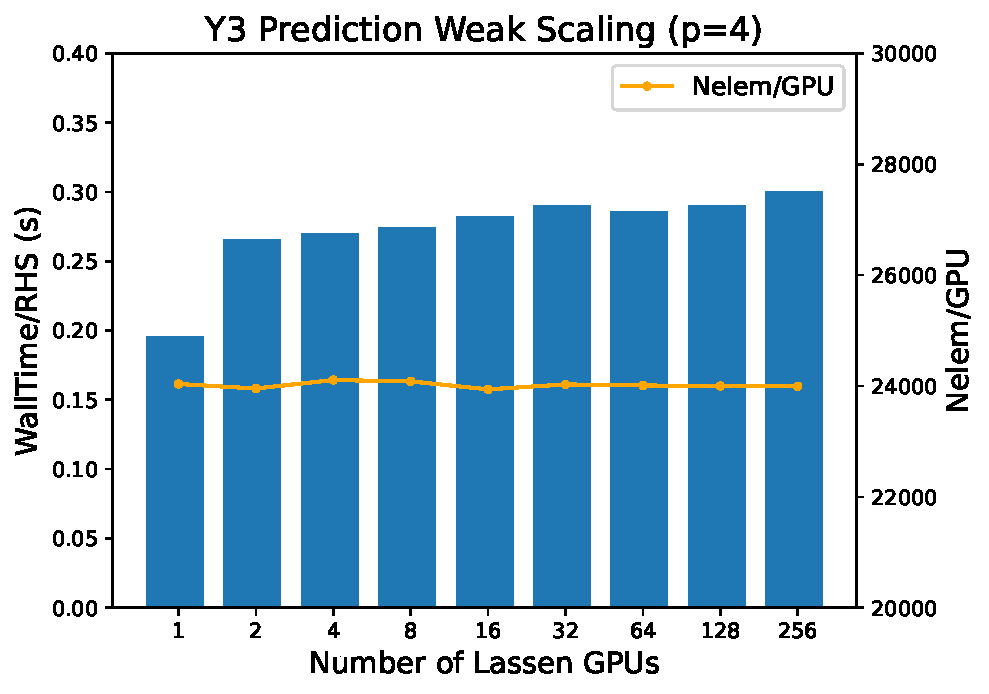
\includegraphics[width=.48\textwidth]{Figures/mtc/y3-prediction_weak_scaling.pdf}
\end{minipage}
\end{frame}

\begin{frame}\frametitle{Prediction Performance Snapshots: Lassen DAT}
    \begin{columns}[T]  % [T] is for top vertical alignment
    % Left Column
    \begin{column}{0.5\textwidth}
      % Top left: Text
      \begin{itemize}
        \item Weak scaling: 24k $p=4$ per GPU
        \item Fluid: NS-only, 2 species
        \item AV: Fluid + Artificial Viscosity
        \item AVMix: AV + 7 species mixture EOS
        \item AVMixLimit: AVMix + species limiter
        \item FullPhysics: AVMixLimit + PLTransport + Wall
      \end{itemize}
      % Bottom left: RHS Compile Times
      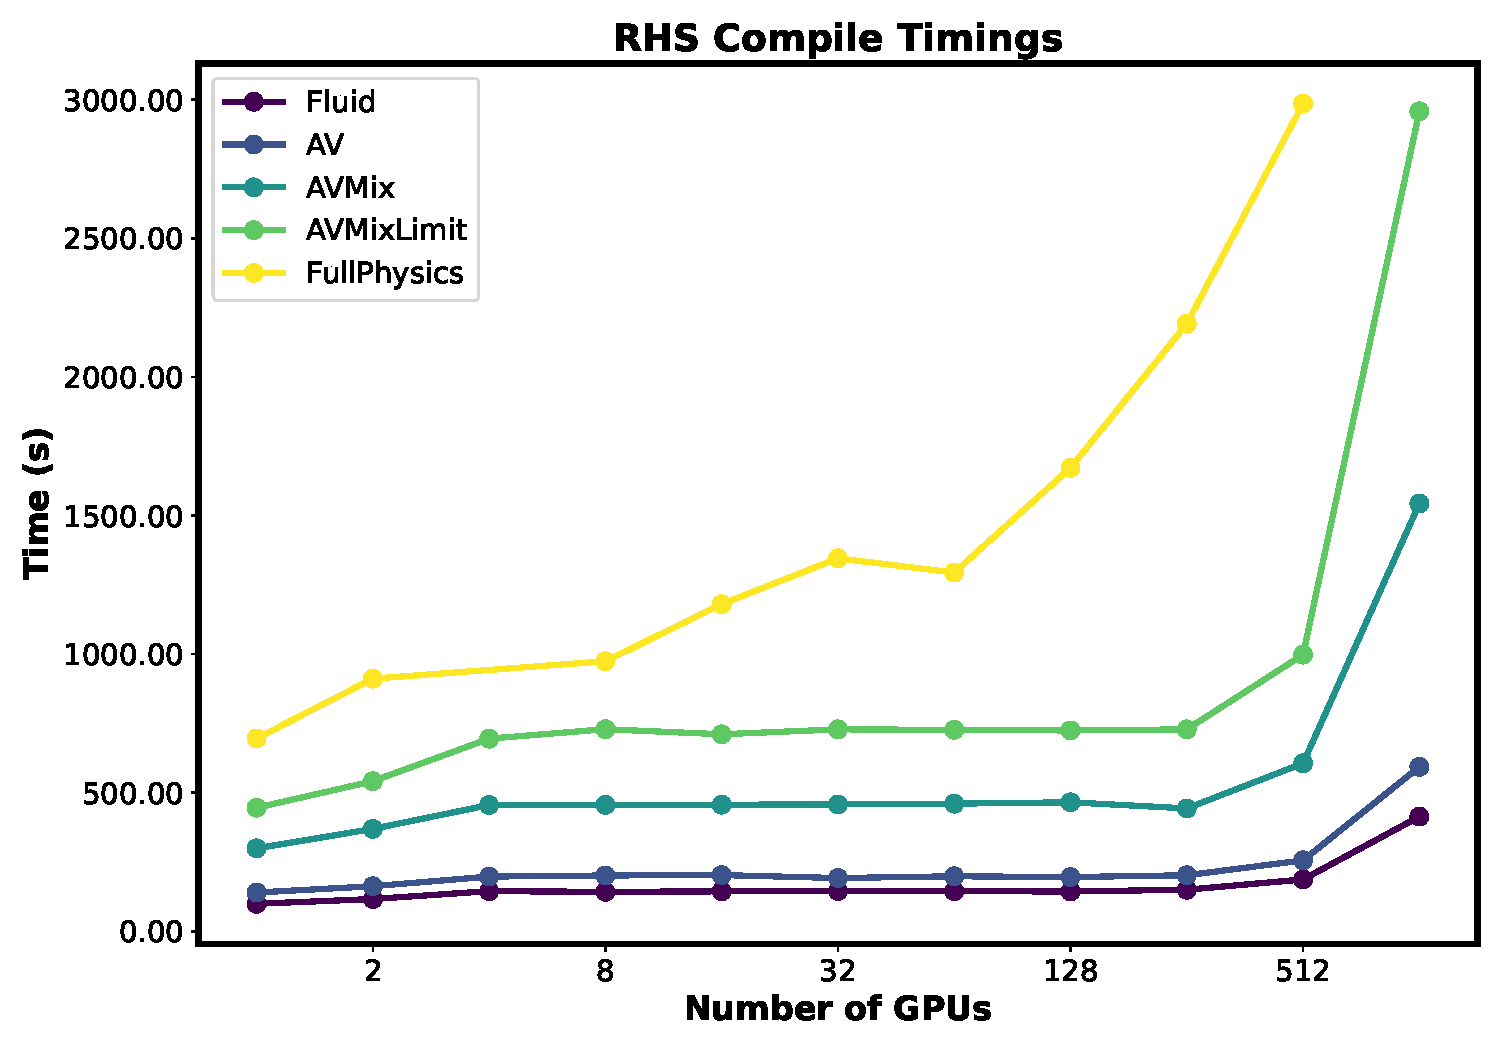
\includegraphics[width=.7\textwidth]{Figures/RHSCompileTimes.pdf}
    \end{column}
    
    % Right Column
    \begin{column}{0.5\textwidth}
      % Top right: Startup Times
      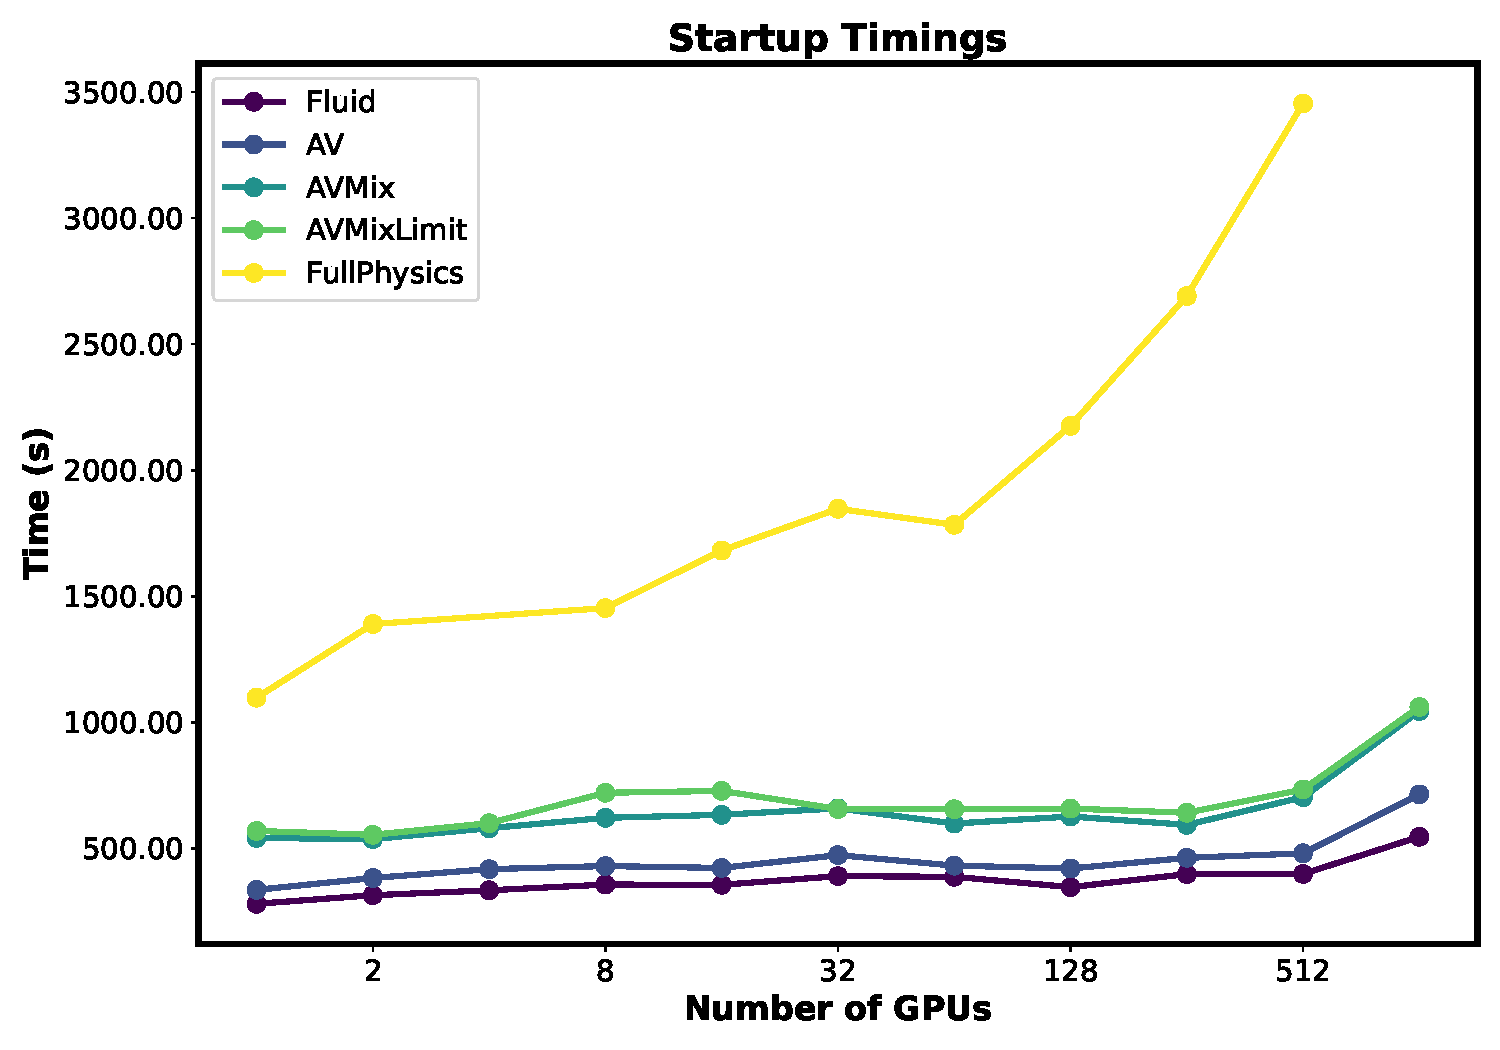
\includegraphics[width=.7\textwidth]{Figures/StartupTimes.pdf}
      % Bottom right: Simulation Step Times
      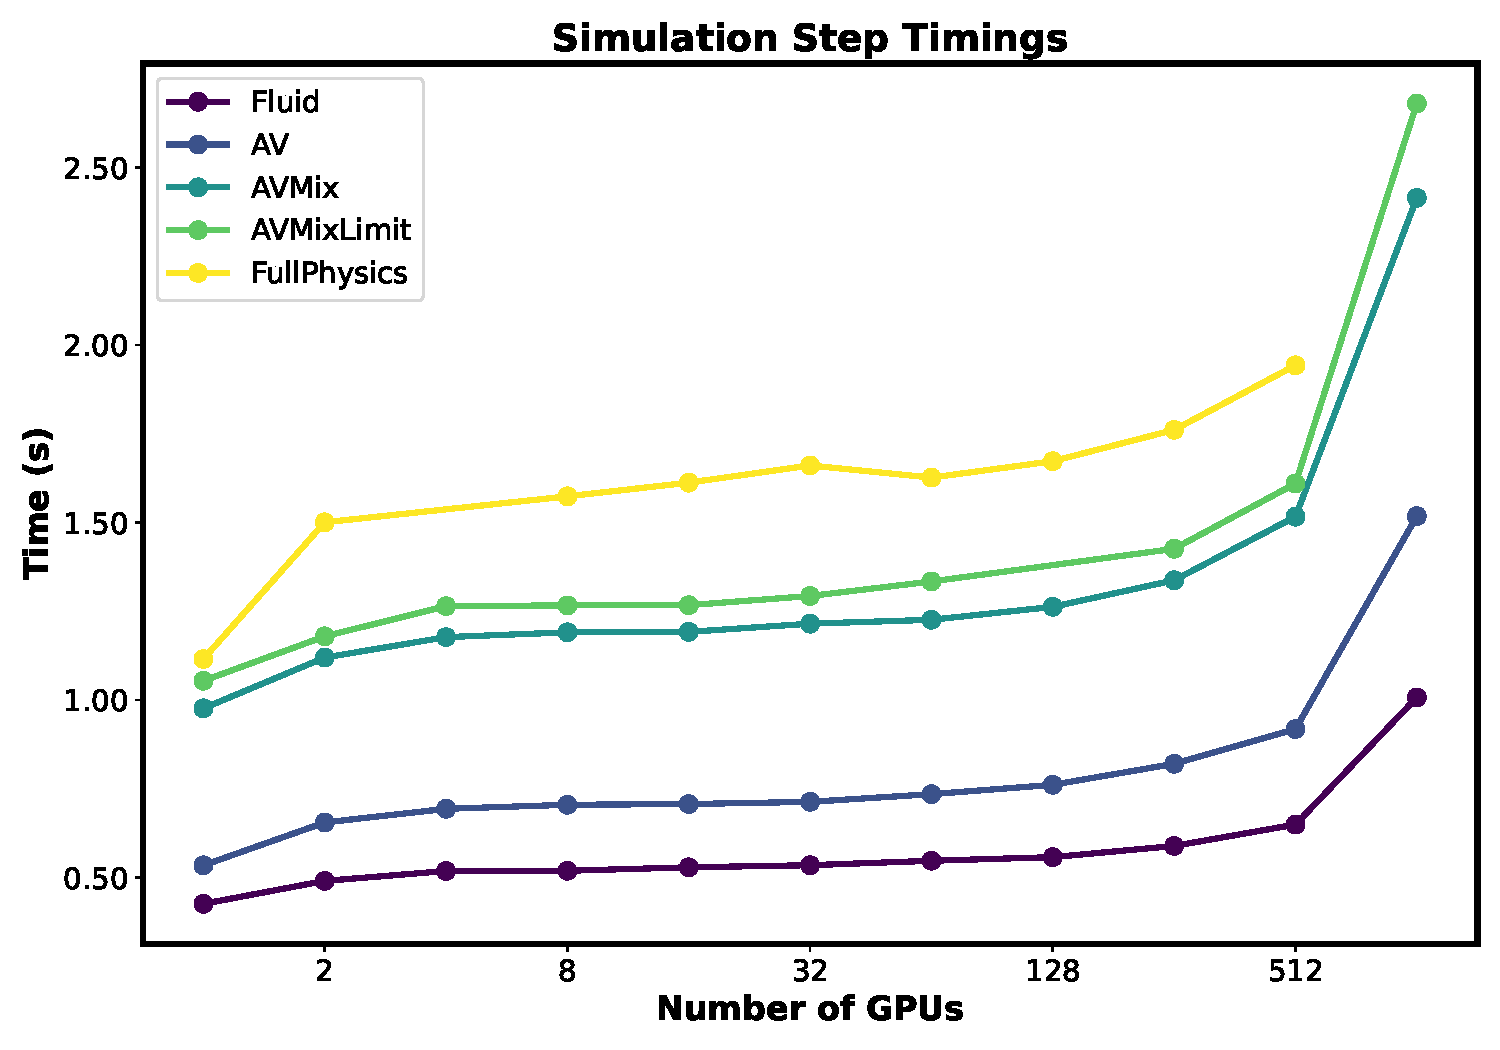
\includegraphics[width=.7\textwidth]{Figures/SimulationStepTimes.pdf}
    \end{column}
  \end{columns}
\end{frame}

%\begin{frame}\frametitle{Prediction Performance Snapshots}
%\end{frame}

%\begin{frame}\frametitle{Prediction Performance Snapshots}
%\end{frame}

\begin{frame}\frametitle{Performance Monitoring on Lassen}
\begin{center}
https://github.com/illinois-ceesd/timing\\
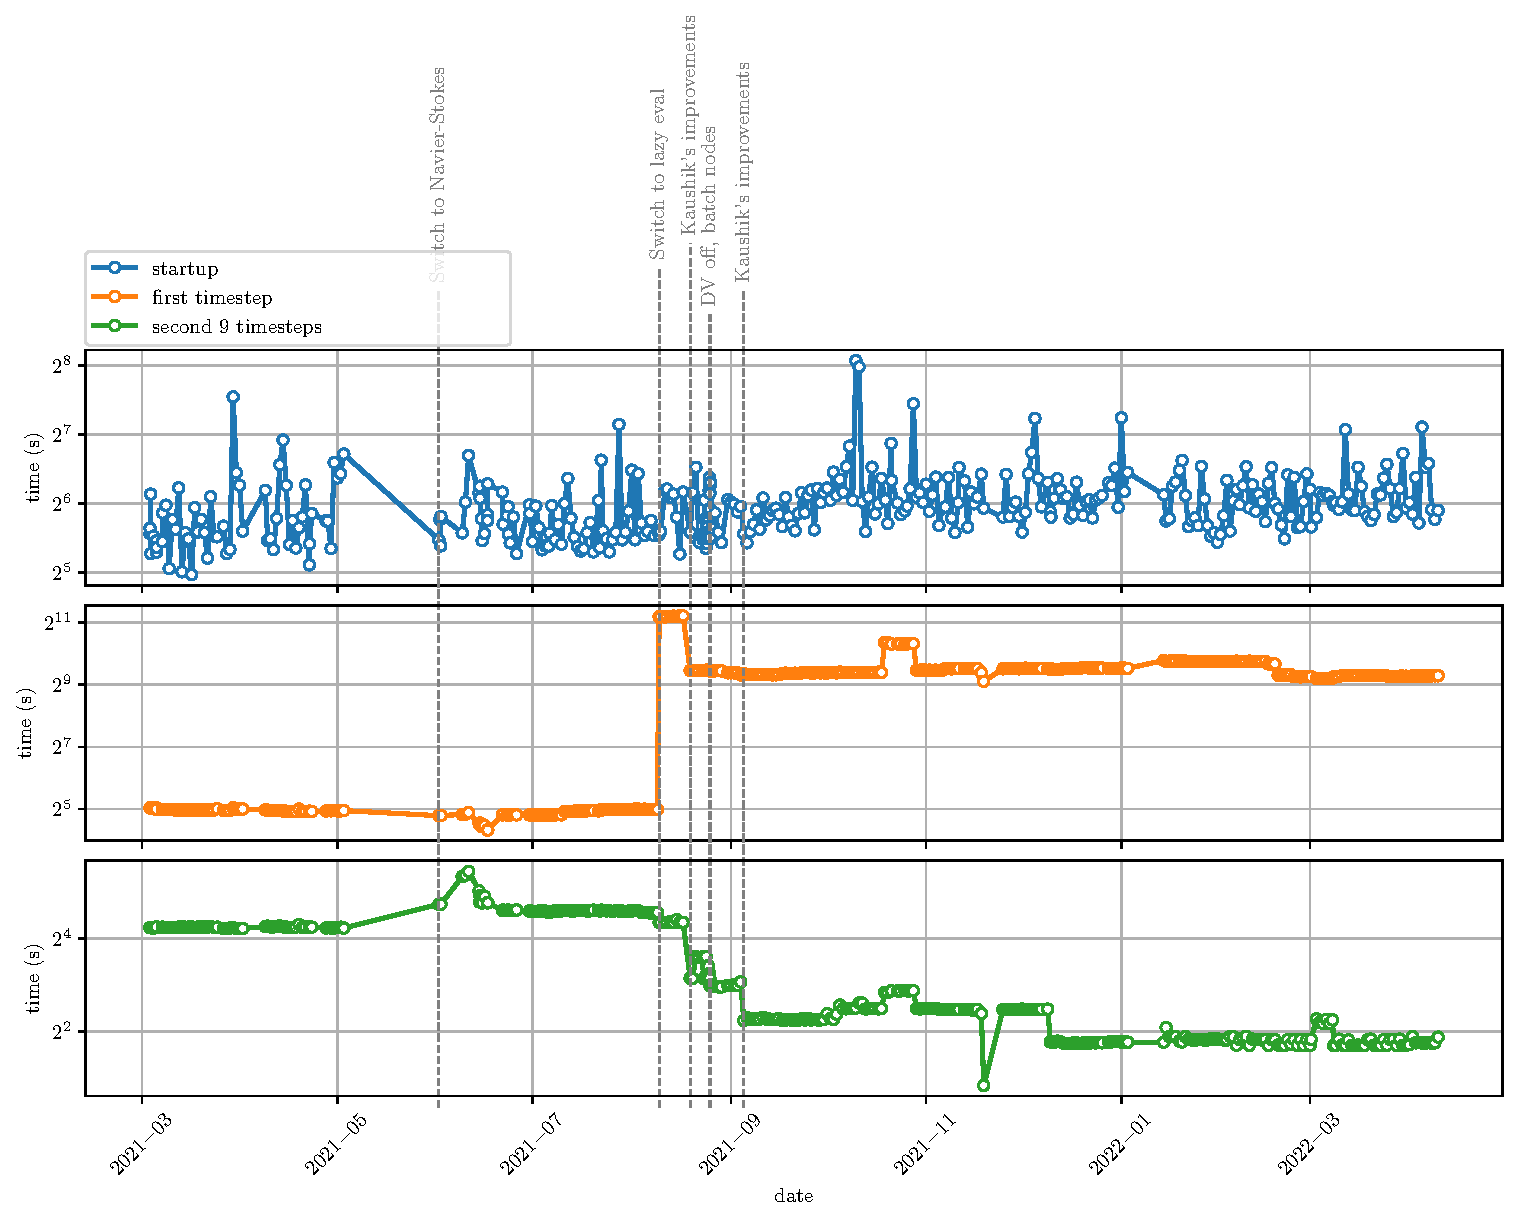
\includegraphics[width=.6\textwidth]{Figures/mtc/nozzle-lazy-full.pdf}
\end{center}
\end{frame}

\begin{frame}\frametitle{Performance Monitoring on Lassen}
\begin{minipage}[t][0.3\textheight][t]{\textwidth}
\begin{center}
https://github.com/illinois-ceesd/timing
\end{center}
\begin{multicols}{2}
\begin{itemize}
\item Data on key capabilities collected nightly
\item Intended to track performance vs. code/features
\item $\Delta$'s indicate change in performance
\columnbreak
\item New this cycle:
\begin{itemize}
\item Multi-case/comparitive plotting
\item Tracking parallel cases
\end{itemize}
\end{itemize}
\end{multicols}
\end{minipage}\vfill
\begin{center}
  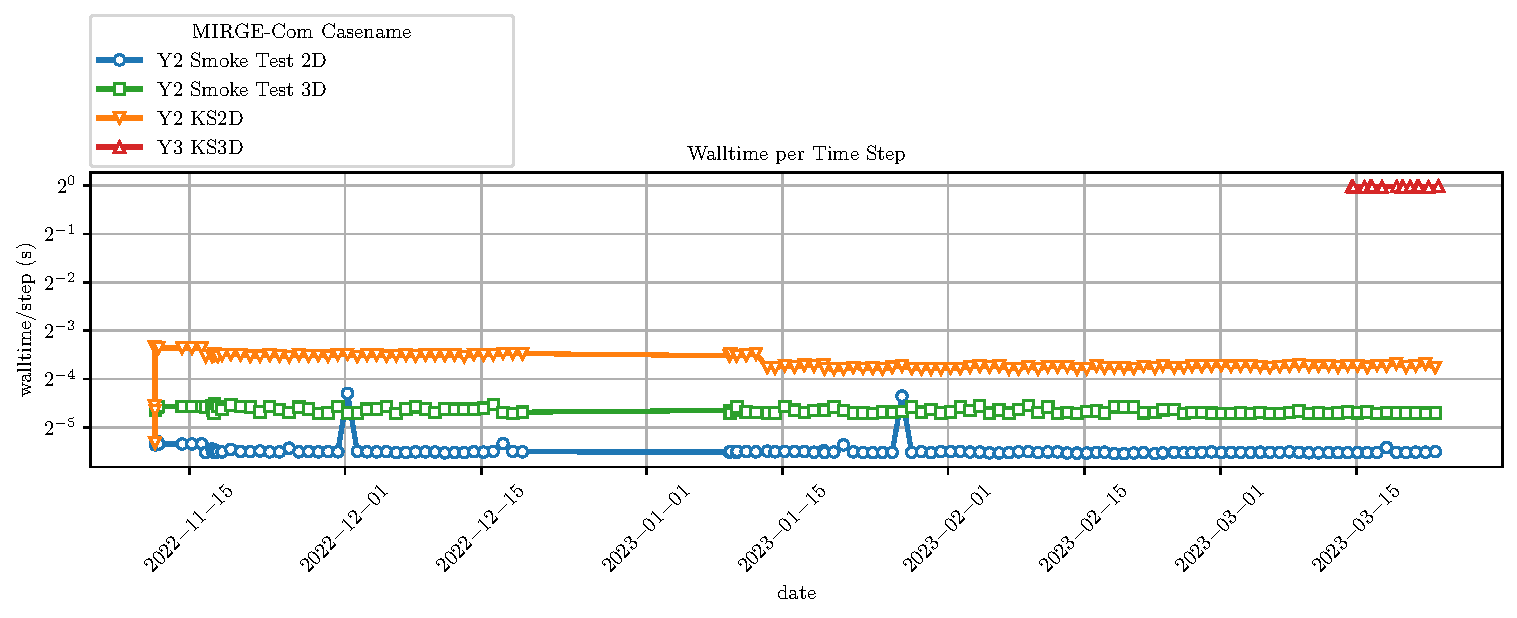
\includegraphics[width=.8\textwidth]{Figures/mtc/multicase_step.pdf}
\end{center}
\end{frame}

\begin{frame}\frametitle{Performance Monitoring on Lassen}
\begin{minipage}[t][0.3\textheight][t]{\textwidth}
\begin{center}
https://github.com/illinois-ceesd/timing
\end{center}
\begin{multicols}{2}
\begin{itemize}
\item Data on key capabilities collected nightly
\item Intended to track performance vs. code/features
\item $\Delta$'s indicate change in performance
\columnbreak
\item New this cycle:
\begin{itemize}
\item Multi-case/comparitive plotting
\item Tracking parallel cases
\end{itemize}
\end{itemize}
\end{multicols}
\end{minipage}\vfill
\begin{center}
  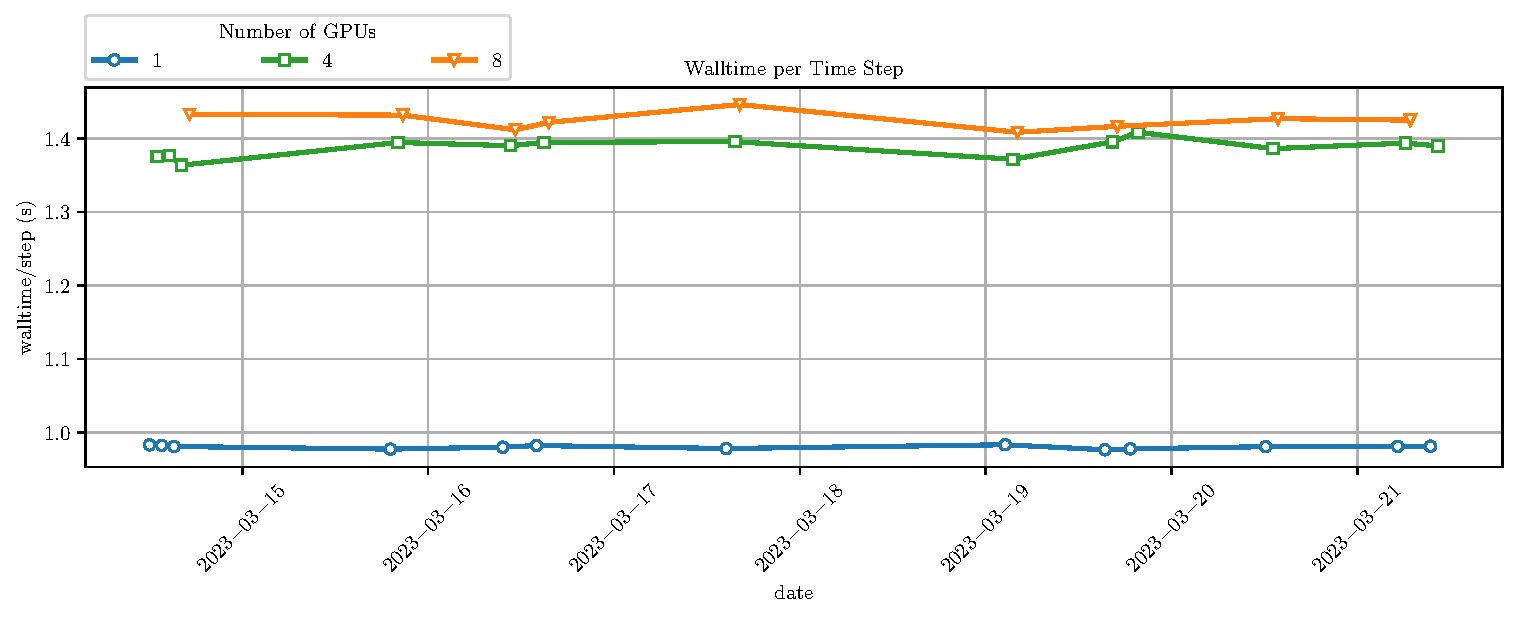
\includegraphics[width=.8\textwidth]{Figures/mtc/prediction-scaling-tracking.pdf}
\end{center}
\end{frame}

\begin{frame}\frametitle{Performance Monitoring on Lassen}
\begin{minipage}[t][0.3\textheight][t]{\textwidth}
\begin{center}
https://github.com/illinois-ceesd/timing
\end{center}
\begin{multicols}{2}
\begin{itemize}
\item Data on key capabilities collected nightly
\item Intended to track performance vs. code/features
\item $\Delta$'s indicate change in performance
\columnbreak
\item New this cycle:
\begin{itemize}
\item Multi-case/comparitive plotting
\item Tracking parallel cases
\end{itemize}
\end{itemize}
\end{multicols}
\end{minipage}\vfill
\begin{center}
  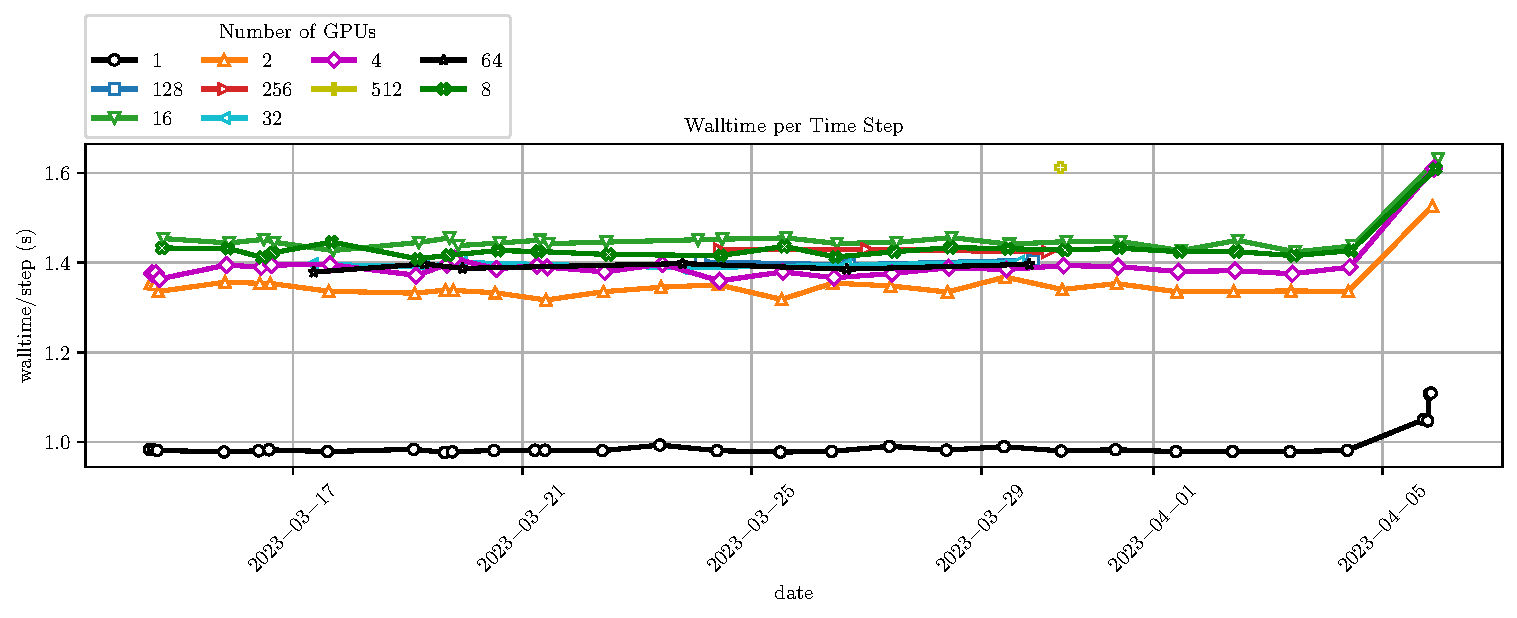
\includegraphics[width=.8\textwidth]{Figures/mtc/y3-prediction-parallel-20230405.pdf}
\end{center}
\end{frame}

\begin{frame}
    \centering
    \Large
    Recent Challenges
\end{frame}

\begin{frame}\frametitle{Recent Challenges and Looming Threats}
\begin{itemize}
\item Loop nest error and indeterminism \prj{\tiny}{M.~Diener, M.~Smith}
\item DAG splat - 1D part seen as looming threat
\item Super long compile times for essential models
\item Mesh I/O and processing
\begin{itemize}
\item Mesh distribution fell down at scale (mpi4py@pkl5)\prj{\tiny}{M.~Diener}
\item Gmsh ingest uses far too much memory
\begin{itemize}
\item Prevented prediction scaling past 512 ranks, precluded machine-scale runs
\item Pre-partitioning work-around gets us to 1024, will 2048 test today!
\end{itemize}
\end{itemize}
\item M-to-N restart: needed for simulation portability (now working for prediction)
\end{itemize}
\end{frame}


\begin{frame}\frametitle{M-to-N Restarts - Single Volume}

\begin{tikzpicture}[scale=0.3]
    \begin{scope}
    % Grid
    \draw[step=1, thin, black] (0,0) grid (16,10);
    \draw[thick] (0,0) rectangle (16,10);
    \end{scope}
\end{tikzpicture}
\end{frame}

\begin{frame}\frametitle{M-to-N Restarts - Single Volume}
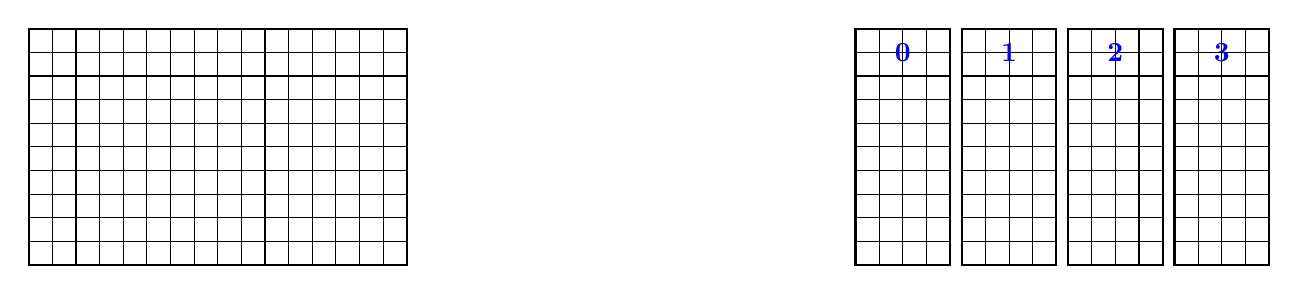
\begin{tikzpicture}[scale=0.3]
    \begin{scope}
    % Grid
    \draw[step=1, thin, black] (0,0) grid (16,10);
    \draw[thick] (0,0) rectangle (16,10);
    \end{scope}

    \begin{scope}[xshift=35cm]
    % Partition 0
    \draw[step=1, thin, black] (0,0) grid (4,10);
    \draw[thick] (0,0) rectangle (4,10);
    \node[font=\bfseries, blue] at (2,9) {0};
    
    % Partition 1
    \begin{scope}[xshift=4.5cm]
        \draw[step=1, thin, black] (0,0) grid (4,10);
        \draw[thick] (0,0) rectangle (4,10);
        \node[font=\bfseries, blue] at (2,9) {1};
    \end{scope}
    
    % Partition 2 with blue and red subregions
    \begin{scope}[xshift=9cm]
        \draw[step=1, thin, black] (0,0) grid (4,10);
        \draw[thick] (0,0) rectangle (4,10);
        % \foreach \j in {0, 1, 2} {
        %    \fill[blue] (1.5, \j+0.5) circle (4pt);
        %    \fill[blue] (2.5, \j+0.5) circle (4pt);
        %    \fill[red] (3.5, \j+0.5) circle (4pt);
        %}
        \node[font=\bfseries, blue] at (2,9) {2};
    \end{scope}
    
    % Partition 3 with red subregion
    \begin{scope}[xshift=13.5cm]
        \draw[step=1, thin, black] (0,0) grid (4,10);
        \draw[thick] (0,0) rectangle (4,10);
        %\foreach \j in {0, 1, 2} {
        %    \fill[red] (0.5, \j+0.5) circle (4pt);
        %    \fill[red] (1.5, \j+0.5) circle (4pt);
        %    \fill[red] (2.5, \j+0.5) circle (4pt);
        %    \fill[red] (3.5, \j+0.5) circle (4pt);
        %}
        \node[font=\bfseries, blue] at (2,9) {3};
    \end{scope}
    \end{scope}
\end{tikzpicture}
\end{frame}

\begin{frame}\frametitle{M-to-N Restarts}
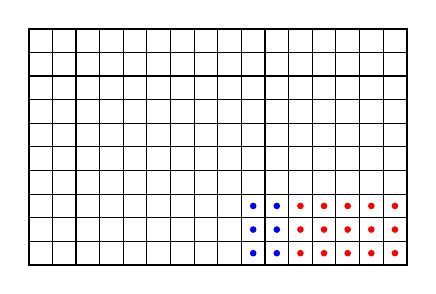
\begin{tikzpicture}[scale=0.3]
    % Grid
    \draw[step=1, thin, black] (0,0) grid (16,10);
    \draw[thick] (0,0) rectangle (16,10);
    
    % Red subregion
    \foreach \i in {11, 12, 13, 14, 15} {
        \foreach \j in {0, 1, 2} {
            \fill[red] (\i+0.5, \j+0.5) circle (4pt);
        }
    }
    
    % Blue subregion
    \foreach \i in {9, 10} {
        \foreach \j in {0, 1, 2} {
            \fill[blue] (\i+0.5, \j+0.5) circle (4pt);
        }
    }
\end{tikzpicture}
\end{frame}

\begin{frame}\frametitle{M-to-N Restarts}
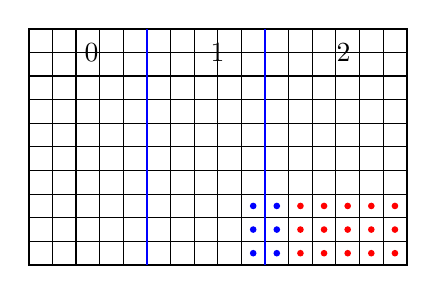
\begin{tikzpicture}[scale=0.3]
    % Grid
    \draw[step=1, thin, black] (0,0) grid (16,10);
    \draw[thick] (0,0) rectangle (16,10);
    
    % Red subregion
    \foreach \i in {11, 12, 13, 14, 15} {
        \foreach \j in {0, 1, 2} {
            \fill[red] (\i+0.5, \j+0.5) circle (4pt);
        }
    }
    
    % Blue subregion
    \foreach \i in {9, 10} {
        \foreach \j in {0, 1, 2} {
            \fill[blue] (\i+0.5, \j+0.5) circle (4pt);
        }
    }

    % Partition lines and labels for 3 partitions
    \draw[thick, blue] (5,0) -- (5,10);
    \draw[thick, blue] (10,0) -- (10,10);
    
    \node at (2.66,9) {0};
    \node at (7.99,9) {1};
    \node at (13.33,9) {2};
\end{tikzpicture}
\end{frame}

\begin{frame}\frametitle{M-to-N Restarts}
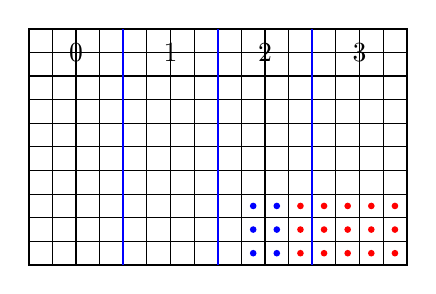
\begin{tikzpicture}[scale=0.3]
    % Grid
    \draw[step=1, thin, black] (0,0) grid (16,10);
    \draw[thick] (0,0) rectangle (16,10);
    
    % Red subregion
    \foreach \i in {11, 12, 13, 14, 15} {
        \foreach \j in {0, 1, 2} {
            \fill[red] (\i+0.5, \j+0.5) circle (4pt);
        }
    }
    
    % Blue subregion
    \foreach \i in {9, 10} {
        \foreach \j in {0, 1, 2} {
            \fill[blue] (\i+0.5, \j+0.5) circle (4pt);
        }
    }

    % Partition lines and labels
    \draw[thick, blue] (4,0) -- (4,10);
    \draw[thick, blue] (8,0) -- (8,10);
    \draw[thick, blue] (12,0) -- (12,10);

    \node at (2,9) {0};
    \node at (6,9) {1};
    \node at (10,9) {2};
    \node at (14,9) {3};
\end{tikzpicture}
\end{frame}


\begin{frame}\frametitle{M-to-N Restarts}
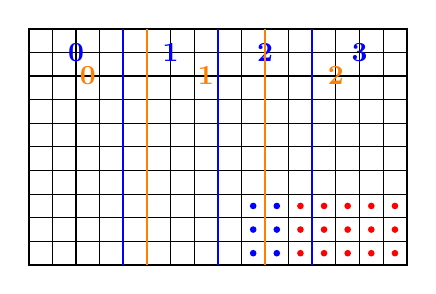
\begin{tikzpicture}[scale=0.3]
    % Grid
    \draw[step=1, thin, black] (0,0) grid (16,10);
    \draw[thick] (0,0) rectangle (16,10);
    
    % Red subregion
    \foreach \i in {11, 12, 13, 14, 15} {
        \foreach \j in {0, 1, 2} {
            \fill[red] (\i+0.5, \j+0.5) circle (4pt);
        }
    }
    
    % Blue subregion
    \foreach \i in {9, 10} {
        \foreach \j in {0, 1, 2} {
            \fill[blue] (\i+0.5, \j+0.5) circle (4pt);
        }
    }

    % Partition lines and labels for 4 partitions (in blue)
    \draw[thick, blue] (4,0) -- (4,10);
    \draw[thick, blue] (8,0) -- (8,10);
    \draw[thick, blue] (12,0) -- (12,10);
    
    \node[font=\bfseries, blue] at (2,9) {0};
    \node[font=\bfseries, blue] at (6,9) {1};
    \node[font=\bfseries, blue] at (10,9) {2};
    \node[font=\bfseries, blue] at (14,9) {3};

    % Partition lines for 3 partitions (in orange)
    \draw[thick, orange] (5,0) -- (5,10);
    \draw[thick, orange] (10,0) -- (10,10);
    
    \node[font=\bfseries, orange] at (2.5,8) {0};
    \node[font=\bfseries, orange] at (7.5,8) {1};
    \node[font=\bfseries, orange] at (13,8) {2};
\end{tikzpicture}
\end{frame}

\begin{frame}
\frametitle{M-to-N Restart}
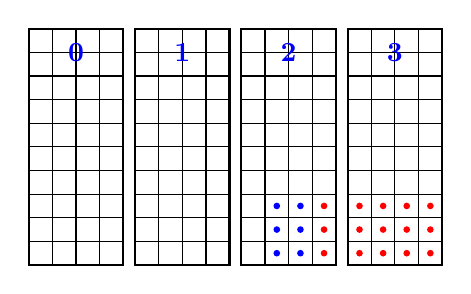
\begin{tikzpicture}[scale=0.3]

    % Partition 0
    \draw[step=1, thin, black] (0,0) grid (4,10);
    \draw[thick] (0,0) rectangle (4,10);
    \node[font=\bfseries, blue] at (2,9) {0};
    
    % Partition 1
    \begin{scope}[xshift=4.5cm]
        \draw[step=1, thin, black] (0,0) grid (4,10);
        \draw[thick] (0,0) rectangle (4,10);
        \node[font=\bfseries, blue] at (2,9) {1};
    \end{scope}
    
    % Partition 2 with blue and red subregions
    \begin{scope}[xshift=9cm]
        \draw[step=1, thin, black] (0,0) grid (4,10);
        \draw[thick] (0,0) rectangle (4,10);
        \foreach \j in {0, 1, 2} {
            \fill[blue] (1.5, \j+0.5) circle (4pt);
            \fill[blue] (2.5, \j+0.5) circle (4pt);
            \fill[red] (3.5, \j+0.5) circle (4pt);
        }
        \node[font=\bfseries, blue] at (2,9) {2};
    \end{scope}
    
    % Partition 3 with red subregion
    \begin{scope}[xshift=13.5cm]
        \draw[step=1, thin, black] (0,0) grid (4,10);
        \draw[thick] (0,0) rectangle (4,10);
        \foreach \j in {0, 1, 2} {
            \fill[red] (0.5, \j+0.5) circle (4pt);
            \fill[red] (1.5, \j+0.5) circle (4pt);
            \fill[red] (2.5, \j+0.5) circle (4pt);
            \fill[red] (3.5, \j+0.5) circle (4pt);  % added this line for the last column of red dots in partition 3
        }
        \node[font=\bfseries, blue] at (2,9) {3};
    \end{scope}
\end{tikzpicture}
\end{frame}

\begin{frame}
\frametitle{M-to-N Restart}
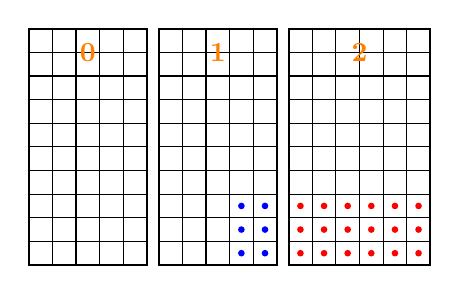
\begin{tikzpicture}[scale=0.3]

    % Partition 0
    \draw[step=1, thin, black] (0,0) grid (5,10);
    \draw[thick] (0,0) rectangle (5,10);
    \node[font=\bfseries, orange] at (2.5,9) {0};
    
    % Partition 1 with blue subregion
    \begin{scope}[xshift=5.5cm]
        \draw[step=1, thin, black] (0,0) grid (5,10);
        \draw[thick] (0,0) rectangle (5,10);
        \foreach \j in {0, 1, 2} {
            \fill[blue] (3.5, \j+0.5) circle (4pt);
            \fill[blue] (4.5, \j+0.5) circle (4pt);
        }
        \node[font=\bfseries, orange] at (2.5,9) {1};
    \end{scope}
    
    % Partition 2 with red subregion
    \begin{scope}[xshift=11cm]
        \draw[step=1, thin, black] (0,0) grid (6,10);
        \draw[thick] (0,0) rectangle (6,10);
        \foreach \j in {0, 1, 2} {
            \fill[red] (0.5, \j+0.5) circle (4pt);
            \fill[red] (1.5, \j+0.5) circle (4pt);
            \fill[red] (2.5, \j+0.5) circle (4pt);
            \fill[red] (3.5, \j+0.5) circle (4pt);
            \fill[red] (4.5, \j+0.5) circle (4pt);
            \fill[red] (5.5, \j+0.5) circle (4pt);
        }
        \node[font=\bfseries, orange] at (3,9) {2};
    \end{scope}
\end{tikzpicture}
\end{frame}

%\begin{frame}
%\frametitle{Grid without Border on Cutout}
%\begin{tikzpicture}[scale=0.3]
%
%    % Draw only the visible cells
%    \foreach \i in {0,1,2,3} {
%        \foreach \j in {3,4,...,9} {
%            \draw (\i,\j) rectangle (\i+1,\j+1);
%        }
%    }
%    \draw (0,0) rectangle (1,3);
%    \draw (0,0) rectangle (1,1);
%    \draw (0,1) rectangle (1,2);
%    \draw (0,2) rectangle (1,3);
%
%    % Adjusted border
%    \draw[thick] (0,0) -- (1,0) -- (1,3) -- (4,3) -- (4,10) -- (0,10) -- cycle;
%
%\end{tikzpicture}
%\end{frame}

\begin{frame}
\frametitle{M-to-N Restart}
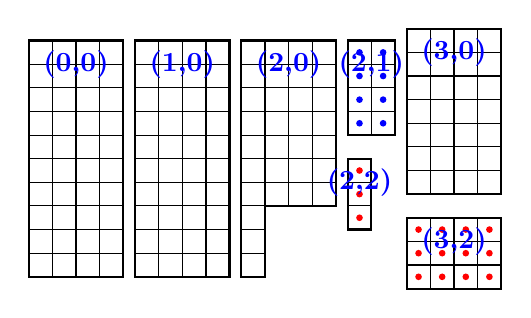
\begin{tikzpicture}[scale=0.3]

    % Partition (0,0)
    \draw[step=1, thin, black] (0,0) grid (4,10);
    \draw[thick] (0,0) rectangle (4,10);
    \node[font=\bfseries, blue] at (2,9) {(0,0)};

    % Partition (1,0)
    \begin{scope}[xshift=4.5cm]
        \draw[step=1, thin, black] (0,0) grid (4,10);
        \draw[thick] (0,0) rectangle (4,10);
        \node[font=\bfseries, blue] at (2,9) {(1,0)};
    \end{scope}

    % Partition (2,0) with the correct shape and border
    \begin{scope}[xshift=9cm]
        \foreach \i in {0,1,2,3} {
            \foreach \j in {3,4,...,9} {
                \draw (\i,\j) rectangle (\i+1,\j+1);
            }
        }
        \draw (0,0) rectangle (1,3);
        \draw (0,0) rectangle (1,1);
v        \draw (0,1) rectangle (1,2);
        \draw (0,2) rectangle (1,3);
        \draw[thick] (0,0) -- (1,0) -- (1,3) -- (4,3) -- (4,10) -- (0,10) -- cycle;
        \node[font=\bfseries, blue] at (2,9) {(2,0)};
    \end{scope}

    % Partition (2,1) with blue subregion, adjusted position
    \begin{scope}[xshift=13.5cm, yshift=6cm]
        \draw[step=1, thin, black] (0,0) grid (2,4);
        \draw[thick] (0,0) rectangle (2,4);
        \foreach \j in {0,1,2,3} {
            \fill[blue] (0.5, \j+0.5) circle (4pt);
            \fill[blue] (1.5, \j+0.5) circle (4pt);
        }
        \node[font=\bfseries, blue] at (1,3) {(2,1)};
    \end{scope}

    % Partition (2,2) with red subregion, adjusted position
    \begin{scope}[xshift=13.5cm, yshift=2cm]
        \draw[step=1, thin, black] (0,0) grid (1,3);
        \draw[thick] (0,0) rectangle (1,3);
        \foreach \j in {0,1,2} {
            \fill[red] (0.5, \j+0.5) circle (4pt);
        }
        \node[font=\bfseries, blue] at (0.5,2) {(2,2)};
    \end{scope}

    % Partition (3,0), adjusted position and dimensions
    \begin{scope}[xshift=16cm, yshift=3.5cm]
        \draw[step=1, thin, black] (0,0) grid (4,7);
        \draw[thick] (0,0) rectangle (4,7);
        \node[font=\bfseries, blue] at (2,6) {(3,0)};
    \end{scope}

    % Partition (3,2) with red subregion, adjusted position
    \begin{scope}[xshift=16cm, yshift=-0.5cm]
        \draw[step=1, thin, black] (0,0) grid (4,3);
        \draw[thick] (0,0) rectangle (4,3);
        \foreach \j in {0,1,2} {
            \fill[red] (0.5, \j+0.5) circle (4pt);
            \fill[red] (1.5, \j+0.5) circle (4pt);
            \fill[red] (2.5, \j+0.5) circle (4pt);
            \fill[red] (3.5, \j+0.5) circle (4pt);
        }
        \node[font=\bfseries, blue] at (2,2) {(3,2)};
    \end{scope}

\end{tikzpicture}
\end{frame}

\begin{frame}
\frametitle{M-to-N Restart}
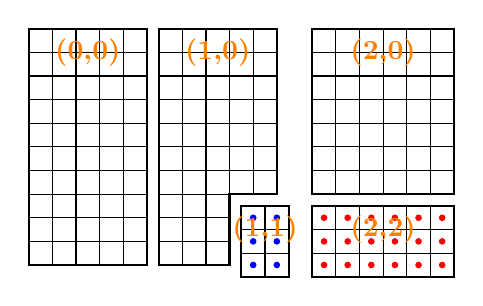
\begin{tikzpicture}[scale=0.3]

    % Partition (0,0)
    \draw[step=1, thin, black] (0,0) grid (5,10);
    \draw[thick] (0,0) rectangle (5,10);
    \node[font=\bfseries, orange] at (2.5,9) {(0,0)};

    % Partition (1,0) with the correct shape, border, and panhandle grid
    \begin{scope}[xshift=5.5cm]
        \foreach \i in {0,1,2,3,4} {
            \foreach \j in {3,4,...,9} {
                \draw (\i,\j) rectangle (\i+1,\j+1);
            }
        }
        \foreach \i in {0,1,2} {
            \foreach \j in {0,1,2} {
                \draw (\i,\j) rectangle (\i+1,\j+1);
            }
        }
        \draw[thick] (0,0) -- (3,0) -- (3,3) -- (5,3) -- (5,10) -- (0,10) -- cycle;
        \node[font=\bfseries, orange] at (2.5,9) {(1,0)};
    \end{scope}

    % Partition (1,1) with blue subregion, further adjusted position
    \begin{scope}[xshift=9cm, yshift=-0.5cm]
        \draw[step=1, thin, black] (0,0) grid (2,3);
        \draw[thick] (0,0) rectangle (2,3);
        \foreach \j in {0,1,2} {
            \fill[blue] (0.5, \j+0.5) circle (4pt);
            \fill[blue] (1.5, \j+0.5) circle (4pt);
        }
        \node[font=\bfseries, orange] at (1,2) {(1,1)};
    \end{scope}

    % Partition (2,0)
    \begin{scope}[xshift=12cm, yshift=3cm]
        \draw[step=1, thin, black] (0,0) grid (6,7);
        \draw[thick] (0,0) rectangle (6,7);
        \node[font=\bfseries, orange] at (3,6) {(2,0)};
    \end{scope}

    % Partition (2,2) with red subregion
    \begin{scope}[xshift=12cm, yshift=-0.5cm]
        \draw[step=1, thin, black] (0,0) grid (6,3);
        \draw[thick] (0,0) rectangle (6,3);
        \foreach \j in {0,1,2} {
            \fill[red] (0.5, \j+0.5) circle (4pt);
            \fill[red] (1.5, \j+0.5) circle (4pt);
            \fill[red] (2.5, \j+0.5) circle (4pt);
            \fill[red] (3.5, \j+0.5) circle (4pt);
            \fill[red] (4.5, \j+0.5) circle (4pt);
            \fill[red] (5.5, \j+0.5) circle (4pt);
        }
        \node[font=\bfseries, orange] at (3,2) {(2,2)};
    \end{scope}

\end{tikzpicture}
\end{frame}

\begin{frame}
\frametitle{M-to-N Restart}

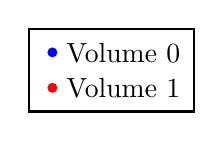
\begin{tikzpicture}[scale=0.3]
    % ... [rest of your existing TikZ picture]

    % Legend Box
    \begin{scope}[xshift=20cm, yshift=8cm]
        \draw[thick] (-1,0.5) rectangle (6,-3); % Adjusted the top border of the box
        
        \fill[blue] (0,-0.5) circle (6pt); % Blue dot
        \node[align=left] at (3,-0.5) {Volume 0}; % Moved the label to the right
        
        \fill[red] (0,-2) circle (6pt);  % Red dot
        \node[align=left] at (3,-2) {Volume 1}; % Moved the label to the right
    \end{scope}
\end{tikzpicture}
\end{frame}

\begin{frame}\frametitle{M-to-N Restarts}
\end{frame}

\begin{frame}
    \centering
    \Large
    Wrapping Up \& Looking Ahead
\end{frame}


\begin{frame}\frametitle{Summary and Next Steps}
\begin{itemize}
\item \mirgecom{} has Y3 prediction-supporting performance (poised to deliver more)
\item Understanding \mirgecom{} performance is the next major focus
\end{itemize}
\begin{center}
Next steps
\end{center}
\begin{multicols}{2}
\begin{itemize}
\item Understanding and improving performance:
\begin{itemize}
\item Instrumentation (Mem \& Tags) \prj{\tiny}{M.~Diener}
\item Code-to-kernel correspondence improvements: \prj{\tiny}{M.~Diener}
\item Auto-tuning \prj{\tiny}{Nick Christensen}
\item DAG Splat \prj{\tiny}{M. Smith}
\item Performance model
\end{itemize}
\item Upcoming enhancements:
\begin{itemize}
\item Workflow: \textit{Parsl} \prj{\tiny}{D.~Friedel}
\item Hexahedral elements \prj{\tiny}{Addison Alvey-Blanco}
\item M-to-N restart (done!)
\end{itemize}
\end{itemize}
%\columnbreak
%\end{multicols}
%\vspace{-20pt}
%\begin{center}
%  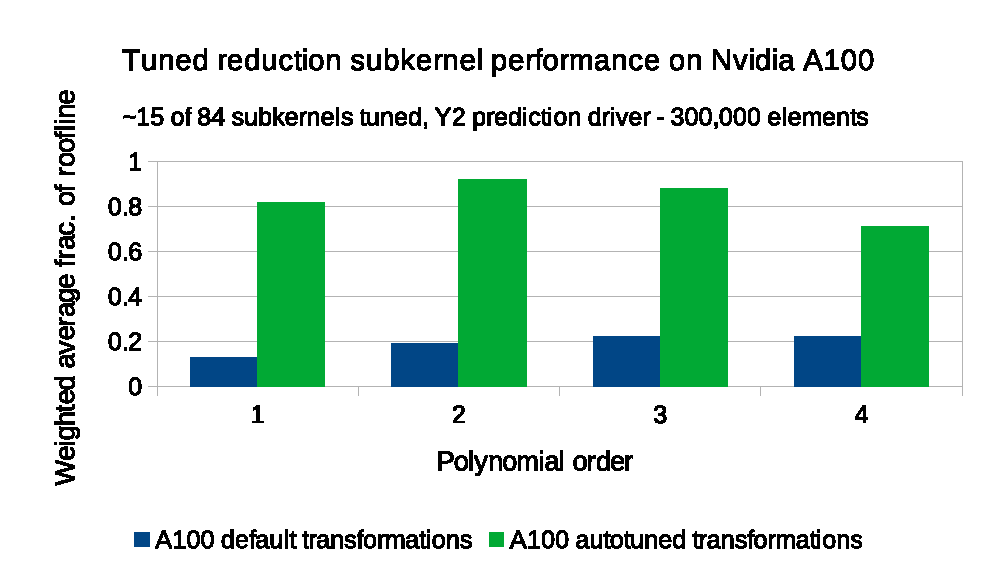
\includegraphics[width=.48\textwidth]{Figures/mtc/Nvidia-A100-performance.eps}
%  \prj{\tiny}{Nick Christensen}
%\end{center}
\end{multicols}
\end{frame}

% - PLANS CHANGE
%\begin{frame}\frametitle{Developments for Y3 Prediction}
%\begin{center}
%Y3 Driver\\
%https://github.com/illinois-ceesd/drivers\_y3-prediction
%\end{center}
%\begin{multicols}{2}
%\begin{itemize}
%\item Kitchen sink (KS) feature set
%  \begin{itemize}
%  \item Coupled CNS + Wall/heat
%  \item Ethylene mixture, reaction sources, species limiting, power-law transport
%  \item Wall degradation, oxygen diffusion, reactive/porous mat.
%  \item Artificial physical viscosity, and sponge
%  \item OFF: Mixture transport, spectral filtering on RHS
 % \end{itemize}
%\item Meshes: 2D/3D updated geom, 2 test sects., shallower cavity
%\item Sims: 3D coupled (6M,p=4 256 GPUs), and smaller
%\item Scalability scripting and inputs (@add-scalability)
%\end{itemize}
%\end{multicols}
%\end{frame}

%\begin{frame}\frametitle{Path to Y3 Prediction}
%\begin{multicols}{2}
%\begin{itemize}
%\item Physics and modeling: Radiation \& Phenolics (mild gap)
%\item Numerics and discretization
%  \begin{itemize}
%  \item Mesh modifications (upstream injector, possible refinement)
%  \item Maybe (gaps suspected):
%    \begin{itemize}
%    \item Higher order mesh + filtering (likely!)
%    \item New AV
%    % \item Slope limiters
%    \item Multi-order meshes/volumes
%    \item ESDG? \prj{\tiny}{Zirui Wang}
%    \item Stop gap: High viscosity, maybe reduced physics
%    \end{itemize}
%  \end{itemize}
%\columnbreak
%\item Performance - closing gaps
%  \begin{itemize}
%  \item Cost per step (inert, comb): (.5, 1.4)s
%  \item Sim time: 1ms inert, 6e-4 w/comb
%  \item Estimated DT: .5ns
%  \item 12d inert, 19d comb
%  \item Any improvements welcomed
%  \end{itemize}
%\end{itemize}
%\end{multicols}
%\end{frame}

%\begin{frame}\frametitle{Path to Y3 Prediction}
%\begin{center}
%\item Preparing for prediction runs
%\end{center}
%\begin{multicols}{2}
%\begin{itemize}
%\item 3M(ish) 3D p=3 elems 
%\item Potentially serious issues: Shock/boundary, fluid/material
%\item Investigating higher order, with filtering, high visc
%\item Many scoping, physics-targeted, and debugging runs
%\end{itemize}
%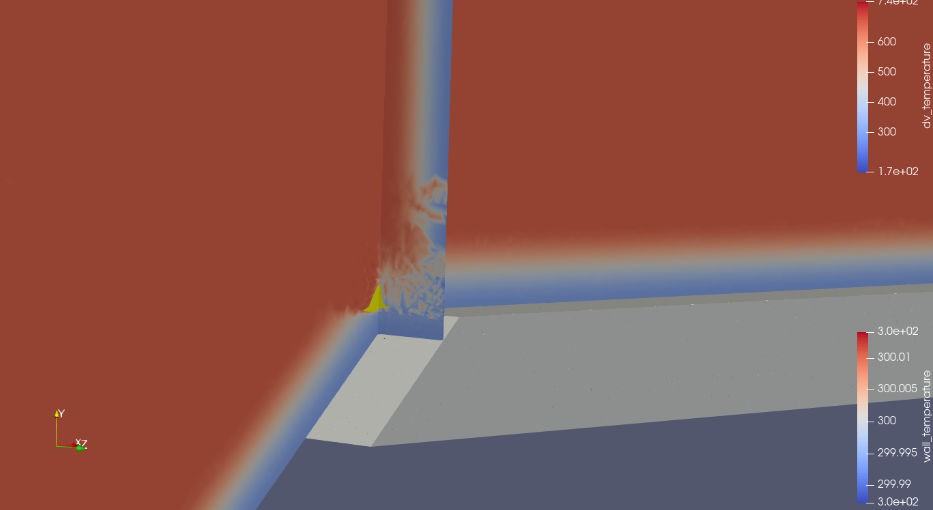
\includegraphics[width=.3\textwidth]{Figures/mtc/hot_edge.png}
%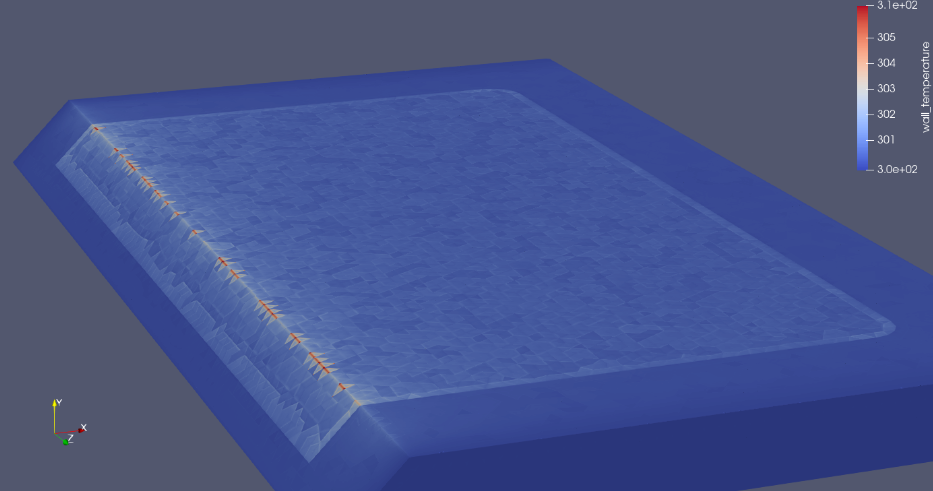
\includegraphics[width=.4\textwidth]{Figures/mtc/3d_yellow_cells.png}
%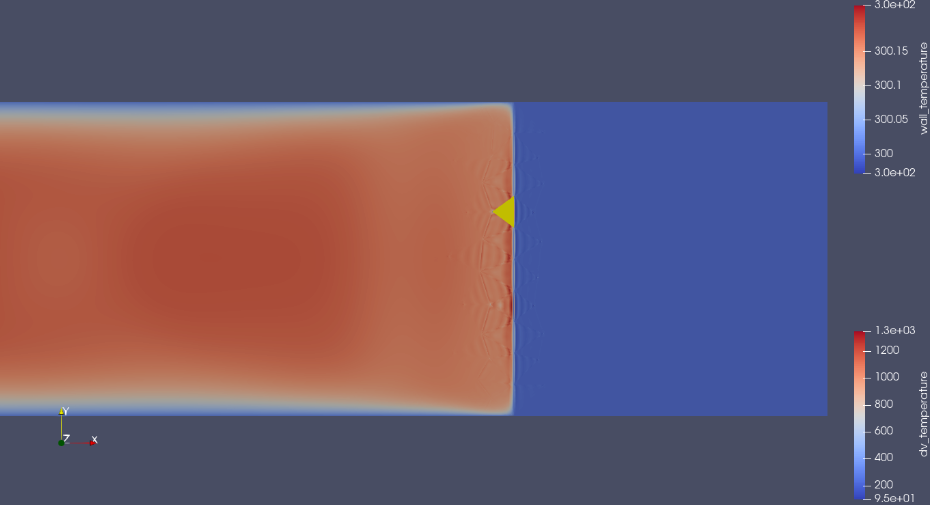
\includegraphics[width=.4\textwidth]{Figures/mtc/2d_yellow_cells.png}
%\end{multicols}
%\end{frame}

%\begin{frame}\frametitle{Path to Y3 Prediction}
%\begin{multicols}{2}
%\begin{itemize}
%\item Some pain points
%  \begin{itemize}
%  \item Transfinite or ultra fine mesh to stabilize fluid boundary
    % \begin{itemize}
    % \item Increases complexity of meshing by a lot
    % \item Increases number of elements
    % \item Hex support desired, might help
    % \end{itemize}
%  \item Lack confidence in correctness of model implementation
    % \begin{itemize}
    % \item Problem with numerics, or defect?
    % \item More extensive testing!
    % \item More experience/intuition about the numerics
    % \item ESDG?, FV?
    % \end{itemize}
%  \item Small problem performance is a drag
    % \begin{itemize}
    % \item 20m compile (this is fine, not fine)
    % \item DAG splat elim, faster compile
    % \end{itemize}
%  \item Makes lots of big files
    % \begin{itemize}
    % \item PARSL
    % \item Viz Driver
    % \end{itemize}
%  \item Development and testing viscosity
%  \item Long queues on available platforms
%  \item Cannot change size of run to adapt to resources
%  \end{itemize}
%\end{itemize}
%\end{multicols}
%\end{frame}


%\begin{frame}\frametitle{Near-term Development Outlook}
%\begin{multicols}{2}
%\begin{itemize}
%\item Now
%  \begin{itemize}
%  \item Understanding performance (why is it hard?)
%    \begin{itemize}
%    \item Code $\leftrightarrow$ Kernel \prj{\tiny}{M.~Diener}
%    \item Performance model
%    \item Kernel rooflines \prj{\tiny}{Nick Christensen}
%    \item Feature-specific
%    \end{itemize}
%  \item Evaluate Tioga
%  \item Boundary verif (MMS)
%  \item PARSL for testing \prj{\tiny}{D.~Friedel}
%  \end{itemize}
%\end{itemize}
%\columnbreak
%\begin{itemize}
%\item For prediction: (4mo horizon)
%  \begin{itemize}
%  \item Radiation \& phenolics \prj{\tiny}{T.~Ricciardi, M.~Smith}
%  \item \sout{DAG splat} \prj{\tiny}{Kaushik Kulkarni}
%  \item Mechanism parameterization for UQ
%  \item PARSL for UQ \prj{\tiny}{D.~Friedel}
%  \item Stabilizing prediction runs \prj{\tiny}{M.~Anderson}
%    \begin{itemize}
%    \item ESDG \prj{\tiny}{Zirui Wang}
%    \item Mixed-order
%    \item Quad/Hex support \prj{\tiny}{Addison Alvey-Blanco}
%    \item Curvlinear elements
%    \end{itemize}
%  \end{itemize}
%\end{itemize}
%\end{multicols}
%\end{frame}

%\begin{frame}\frametitle{Nice to have any time}
%\begin{multicols}{2}
%\begin{itemize}
%\item Reducing prediction pain (important):
%  \begin{itemize}
%  \item Reduce technical debt (merges)
%  \item Driver unification
%  \item Help with mesh generation
%  \item Visualization driver
%  \item PARSL for queue management
%  \item M-to-N restart
 % \end{itemize}
%%\item Potentially high-impact performance improvements
%  \begin{itemize}
%  \item Kernel Autotuning \prj{\tiny}{Nick Christensen}
%  \item Node-aware communication \prj{\tiny}{Shelby Lockhart}
%  \item DAG/compile time improvements \prj{\tiny}{Kaushik Kulkarni, M.~Diener}
%  \item Instrumentation (Mem \& Tags) \prj{\tiny}{Kaushik Kulkarni, M.~Diener}
%  \end{itemize}
%\item Future sims
%  \begin{itemize}
%  \item Mesh motion (interface regression)
%  \item Wall degradation
%  \item Turbulence modeling
%  \end{itemize}
%\end{itemize}
%\end{multicols}
%\end{frame}

